% =====================================================================
% Governance Drift: Measuring Divergence Between Approved Intent and
% Operational Reality in Cloud-Native Systems
%
% Journal-length manuscript, IEEE-Transactions-style formatting on the
% base article class (content transplants directly into IEEEtran /
% llncs / elsarticle for submission).
% =====================================================================
\newif\ifanonymoussubmission
\ifdefined\GOVDRIFTANONYMOUS
  \anonymoussubmissiontrue
\else
  \anonymoussubmissionfalse
\fi
\documentclass[10pt,twocolumn]{article}
\PassOptionsToPackage{hyphens}{url}

\usepackage[T1]{fontenc}
\usepackage[utf8]{inputenc}
\usepackage{mathptmx}
\usepackage[scaled=0.90]{helvet}
\usepackage{courier}
\usepackage[letterpaper,left=0.66in,right=0.66in,top=0.73in,bottom=0.95in]{geometry}
\setlength{\columnsep}{0.25in}
\usepackage{microtype}

\usepackage{amsmath,amssymb,amsthm}
\usepackage{graphicx}
\usepackage{xcolor}
\usepackage{booktabs}
\usepackage{multirow}
\usepackage{threeparttable}
\usepackage{enumitem}
\usepackage{listings}
\usepackage{caption}
\usepackage{titlesec}
\usepackage{tikz}
\usetikzlibrary{arrows.meta,positioning,calc,shapes.geometric,fit,backgrounds,decorations.pathreplacing,matrix}
\usepackage{flushend}
\usepackage[hidelinks]{hyperref}
\usepackage{url}
\usepackage[capitalize,noabbrev]{cleveref}
\hypersetup{
  pdftitle={Governance Drift: Measuring Divergence Between Approved Intent and Operational Reality in Cloud-Native Systems},
  pdfsubject={History-anchored governance-drift measurement in cloud-native systems},
  pdfkeywords={governance drift, configuration drift, GitOps, cloud governance, Kubernetes}
}
\ifanonymoussubmission
  \hypersetup{pdfauthor={}}
\else
  \hypersetup{pdfauthor={Obede Bessa Rocha da Silva}}
\fi

\renewcommand{\thesection}{\Roman{section}}
\renewcommand{\thesubsection}{\thesection-\Alph{subsection}}
\renewcommand{\thesubsubsection}{\thesubsection.\arabic{subsubsection}}
\titleformat{\section}{\centering\normalsize\scshape}{\thesection.}{0.5em}{}
\titleformat{\subsection}{\normalsize\itshape}{\Alph{subsection}.}{0.5em}{}
\titleformat{\subsubsection}{\normalsize\itshape}{\arabic{subsubsection})}{0.5em}{}
\titlespacing*{\section}{0pt}{2.2ex plus .6ex minus .2ex}{1.2ex plus .3ex}
\titlespacing*{\subsection}{0pt}{1.8ex plus .5ex minus .2ex}{0.8ex plus .2ex}
\titlespacing*{\subsubsection}{0pt}{1.4ex plus .4ex minus .2ex}{0.6ex plus .2ex}

\captionsetup[figure]{font=footnotesize,labelsep=period,name=Fig.}
\captionsetup[table]{font=footnotesize,labelsep=newline,justification=centering,labelfont=sc,textfont=sc}
\renewcommand{\thetable}{\Roman{table}}

\newtheoremstyle{ieeedef}{0.7em}{0.7em}{\itshape}{\parindent}{\itshape}{:}{0.4em}{}
\theoremstyle{ieeedef}
\newtheorem{definition}{Definition}
\newtheorem{proposition}{Proposition}
\newtheorem{metricdef}{Metric}
\renewcommand{\themetricdef}{M\arabic{metricdef}}
\newtheorem{finding}{Finding}
\renewcommand{\thefinding}{F\arabic{finding}}
\newtheorem{scenario}{Scenario}
\renewcommand{\thescenario}{S\arabic{scenario}}
\crefname{definition}{Definition}{Definitions}
\crefname{proposition}{Proposition}{Propositions}
\crefname{metricdef}{Metric}{Metrics}
\crefname{finding}{Finding}{Findings}
\crefname{scenario}{Scenario}{Scenarios}

\definecolor{lstbg}{gray}{0.97}
\lstset{
  basicstyle=\ttfamily\fontsize{7.2}{8.6}\selectfont,
  breaklines=true, breakatwhitespace=true,
  frame=single, framerule=0.3pt, rulecolor=\color{black!50},
  backgroundcolor=\color{lstbg},
  xleftmargin=4pt, xrightmargin=4pt,
  aboveskip=6pt, belowskip=4pt,
  showstringspaces=false, columns=fullflexible, keepspaces=true
}

% ------------------------- math macros -------------------------------
\newcommand{\Gapp}{G_{\mathrm{app}}}
\newcommand{\Gobs}{G_{\mathrm{obs}}}
\newcommand{\Pol}{\mathcal{P}}
\newcommand{\Auth}{\mathcal{A}}
\newcommand{\Int}{\mathcal{I}}
\newcommand{\Evd}{\mathcal{E}}
\newcommand{\GD}{\mathsf{GD}}
\newcommand{\GDsub}{\mathsf{GD}_{\mathrm{sub}}}
\newcommand{\ObsMask}{\mathsf{O}}
\newcommand{\dconf}{d_{\mathrm{conf}}}
\newcommand{\dpol}{d_{\mathrm{pol}}}
\newcommand{\dauth}{d_{\mathrm{auth}}}
\newcommand{\dint}{d_{\mathrm{int}}}
\newcommand{\denv}{d_{\mathrm{env}}}
\newcommand{\devd}{d_{\mathrm{evd}}}
\newcommand{\Cons}{\mathsf{Consistent}}
\newcommand{\dig}{h}
\newcommand{\unk}{\bot}

\tikzset{
  stage/.style={draw=black!70, rounded corners=1.5pt, fill=black!4,
    minimum height=6.5mm, minimum width=14mm, align=center,
    font=\fontsize{7.2}{8.2}\selectfont},
  human/.style={stage, fill=black!5},
  attn/.style={draw=black!70, fill=black!4, rounded corners=1.5pt,
    minimum height=5mm, align=center, font=\fontsize{6.8}{7.9}\selectfont},
  evid/.style={draw=black!70, fill=black!10, rounded corners=1.5pt,
    minimum height=5mm, align=center, font=\fontsize{6.8}{7.9}\selectfont},
  brok/.style={draw=black, densely dashed, fill=black!8, rounded corners=1.5pt,
    minimum height=5mm, align=center, font=\fontsize{6.8}{7.9}\selectfont},
  lbl/.style={font=\fontsize{6.8}{7.9}\selectfont},
  flow/.style={-{Stealth[length=2mm]}, thick},
  eflow/.style={-{Stealth[length=1.6mm]}, densely dashed, black!60},
  bflow/.style={-{Stealth[length=1.6mm]}, black, densely dotted, thick}
}
\newcommand{\smlbl}{\fontsize{6.8}{7.9}\selectfont\color{black!70}}
\newcommand{\cmark}{\ensuremath{\checkmark}}
\newcommand{\xmark}{\ensuremath{\times}}

% =====================================================================
\begin{document}

\twocolumn[{%
\begin{center}
{\fontsize{21}{25}\selectfont
Governance Drift: Measuring Divergence Between Approved\\[2pt]
Intent and Operational Reality in Cloud-Native Systems\par}
\vspace{14pt}
\ifanonymoussubmission
  {\fontsize{11}{13}\selectfont Anonymous Author(s)\par}
\else
  {\fontsize{11}{13}\selectfont Obede Bessa\par}
  \vspace{2pt}
  {\fontsize{9}{11}\selectfont Independent Researcher \;---\; obedebessa@gmail.com\par}
\fi
\vspace{16pt}
\end{center}
}]

% ------------------------- abstract ----------------------------------
\noindent\textbf{\textit{Abstract}---Configuration drift compares desired and observed configuration; it cannot decide whether a running system remains covered by what authorized it. We define \emph{governance drift} as a history-anchored relation among operational reality, current governance context, and a unique activated approval basis. The model separates five substantive components from epistemic observability and specifies stable identity, activation and supersession, and admissible temporal cuts. In a twelve-scenario closed world, a cumulative ablation raises unconditional exact-vector success from 75.0\% for plane-local signals to 100\% for the admitted-basis join. On a version-pinned Kind/Flux/Kyverno stack, 180 injections yielded 538/540 detections and 538/538 exact provisional class sets conditional on detection; 777 benign-transition polls produced no policy, authorization, intent, or environment drift, and all 60 trajectories ended provisionally consistent. A process-isolated audit reached the exact target in 27/27 correlated trajectories: cause-start-to-first-exact completion had median 4.465~s (P95 9.764), and cause-start-to-second-consecutive-exact completion had median 9.522~s (P95 19.811), without a Stable-VCL claim. A separate Argo CD/Gatekeeper replication produced 15/15 exact projected singleton classifications over declared components: S1 configuration and S3 policy used native paths, whereas S4 authorization reused the shared digest adapter. This is neither complete-vector validation nor cross-stack equivalence. The results demonstrate bounded semantic realizability and safe uncertainty handling, not natural prevalence or production effectiveness.}

\vspace{4pt}
\noindent\textbf{\textit{Index Terms}---Governance drift, configuration drift, GitOps, policy as code, cloud governance, Kubernetes, continuous compliance, DevOps, distributed systems.}
\vspace{8pt}

\section{Introduction}
\label{sec:intro}

Reconciliation-based delivery gave cloud operations a powerful invariant:
the running system converges to a declared desired state, and divergence---%
\emph{configuration drift}---is detected and repaired
continuously~\cite{opengitops,beetz2022,argocd,fluxcd,burns2016}. The invariant
is so useful that it has quietly become a proxy for a much stronger claim. When
the reconciler reports \textsc{Synced} and the drift detector reports clean,
operators, auditors, and dashboards read: \emph{the system is in the state we
approved}. This paper is about the gap between those two statements.

Consider a payments service whose deployment was approved on March~3rd: the
manifest matched revision \texttt{rev-42}, satisfied policy version
$\pi_7$, carried a service-owner approval bound to image digest
\texttt{sha256:aaa\ldots}, and traced to ticket \texttt{TKT-99}. Months later
the cluster still matches its Git manifest byte for byte. Meanwhile: the
security team superseded $\pi_7$ with $\pi_8$, which the running configuration
violates; an emergency exception granted during an incident expired
after four hours and has now been silently in force for six weeks; the registry
re-tagged \texttt{svc:1.4.2} so the pods run a digest no approval ever
referenced; and a well-meaning rollback reverted Git to \texttt{rev-37},
content whose approval belongs to a different change. Configuration drift:
zero. One or more legitimacy conditions that covered the deployment on
March~3rd no longer hold. We call this condition \emph{governance drift}: the
operational state has diverged not from its manifest but from the state,
policy context, authorization basis, and intent \emph{under which it was
approved}.

The distinction is not terminological. The desired/observed
configuration-drift signal implemented by reconcilers and commonplace IaC
drift tools is a \emph{two-place, memoryless} relation between two
configurations and is therefore decidable by comparison
\cite{awsconfig,driftctl}. Configuration-management programs can retain
approved historical baselines (\cref{sec:related}), but their decision object
remains configuration-scoped. Governance drift is a
\emph{three-place, history-anchored} relation among present state, evolving
context, and an immutable admitted basis; we establish the separation in two complementary
forms: constructed, tool-realizable counterexamples, and a
definitional-dependency result showing that no detector whose inputs are
configuration pairs---however sophisticated its diffing---can decide
governance consistency, because the deciding facts are not functions of those
inputs (\cref{prop:impossible}). Worse, reconciliation can materialize an
unauthorized desired-state change and then erase the transient
configuration-drift signal, leaving intent drift: the rollback scenario above
is converged into content outside the historically authorized change lineage
(\cref{sec:taxonomy}).

Our executed study makes the separation concrete. We implement a
governance-drift detector evaluated at cumulative evidence tiers---%
configuration comparison; plus policy re-evaluation; plus authorization
records with validity semantics; plus artifact lineage; plus environment
inventory against recorded assumptions---against twelve injected drift
scenarios (including compound drift and evidence decay) and a no-drift control containing both
runtime churn and \emph{benign governance churn} (satisfied policy
revisions, approved updates, hygienic exceptions), under a counterfactual
scoring rule that credits information rather than alarm volume. The result is
a strict detectability staircase (\cref{tab:matrix}): normalized
configuration comparison detects exactly one scenario of twelve; each evidence
tier detects precisely the scenarios whose deciding facts it carries; the
governance tiers achieve zero false alarms \emph{earned against} governance
churn. A deliberately naive unnormalized comparator is retained only as a
scoring diagnostic, not as a production baseline.

\subsection{Research Questions}
\begin{description}[leftmargin=3.2em,itemsep=1pt,topsep=2pt]
\item[RQ0:] Can divergence between approved intent and operational reality be
formally represented and measured as governance drift?
\item[RQ1:] Which forms of governance drift can arise and be distinguished in
cloud-native systems?
\item[RQ2:] Can governance drift be detected using existing operational,
governance, and control-plane evidence streams?
\item[RQ3:] How quickly does governance drift become visible?
\item[RQ4:] Which forms of drift are detectable through configuration
comparison alone, and which require authorization or evidence context?
\end{description}

RQ0 is answered by the formal model and the combined analytic and empirical
results. RQ1 is answered by the taxonomy and scenario catalog
(\cref{sec:taxonomy,sec:study}); RQ2 and RQ4 by the dependency result (\cref{prop:impossible}), the tiered architecture (\cref{sec:architecture}),
the executed detectability study (\cref{sec:study}), and the bounded live
laboratory (\cref{sec:lab}); RQ3 by the study's event-time measurements and
the laboratory's separated actuation, onset-to-detection, end-to-end, and
time-to-evidence observations across three polling cadences.

\subsection{Contributions and Epistemic Status}
\begin{enumerate}[label=\textbf{C\arabic*.},leftmargin=2.2em,itemsep=1.5pt,topsep=2pt]
\item \textbf{Taxonomy} (conceptual): formal definitions separating
five substantive components---configuration, policy, authorization, intent,
and environment---plus transversal epistemic evidence drift, with governance
drift as their umbrella---and with the explicit
commitment that governance drift must not, and provably does not, reduce to
configuration drift (\cref{sec:taxonomy}).
\item \textbf{Formal model} (conceptual/analytic): an immutable sequence of
atomic approval snapshots plus separate activation and supersession records,
stable unit identity, admissible cross-stream temporal cuts, observed state $\Gobs(t)$, time-indexed governance contexts
$\Pol(t), \Auth(t), \Int(t)$, and a component-wise governance-divergence vector
$\GDsub(u,\theta)$ plus an observability mask $\ObsMask_{\mu}(u,\theta;T)$, with a reasoned rejection of a primitive scalar distance
(\cref{sec:model}).
\item \textbf{Separation results} (analytic): constructed counterexamples and
a definitional-dependency proposition establishing that configuration
equality does not imply governance consistency and that no configuration-pair
detector decides it---deliberately elementary, and billed as such
(\cref{sec:taxonomy,sec:model}).
\item \textbf{Detection architecture} (design): a vendor-neutral tiered
architecture mapping each component to a sufficient evidence tier, together
with indistinguishable-world constructions proving tier minimality
(\cref{sec:architecture,prop:tier-minimality}).
\item \textbf{Executed detector study} (empirical, closed-world): twelve
scenarios $\times$ six detector tiers $\times$ twenty seeds, with
counterfactual scoring, full-vector ground truth, three compound scenarios,
exact-set and Hamming scoring, a separately implemented composite comparator without the
admitted-basis join, and a control containing
runtime \emph{and} benign governance churn; all code and data packaged,
matrix generated programmatically (\cref{sec:study}). Its role is precisely
scoped: it validates that the reference semantics realize the model's
dependency structure and quantifies noise behavior; it is not field evidence,
and it makes no claim about any real cluster.
\item \textbf{Repeated Kubernetes/GitOps laboratory} (empirical, executed): a
version-pinned Kind/Flux/Kyverno stack, local Git and OCI services, approved-state
recorder, tiered evaluator, and executable injections for S1--S9. In one
hundred eighty controlled injections (20 per scenario), three randomized-phase
polling cadences produced 538/540 detections and 100\% conditional exact-set
accuracy for provisional class-set classifications under the laboratory's
sequential-snapshot assumption. Twenty steady-state benign windows produced no alarms in 543 polls;
a separate transition-inclusive campaign began three isolated observers before
each benign mutation and retained all 777 polls, including seven expected
configuration-convergence polls and 36 fail-safe epistemic warning polls but
no policy, authorization, intent, or environment drift; all 60 trajectories
ended with a provisionally consistent classification
(\cref{sec:lab}). A secondary S10--S12 extension reached
the exact provisional class set in 45/45 cadence observations; six separate 300-s benign windows
added 4,680 steady-state polls without substantive or epistemic alarms. The execution
demonstrates bounded realizability and behavior within the reported laboratory conditions, not natural occurrence,
prevalence, production effectiveness, stream-loss reliability, or transfer.
\item \textbf{Boundary campaigns} (empirical, executed): a nine-episode audit
with 27 separate observer processes and 261 raw polls; nine controlled profiles
through a two-hop localhost TCP evidence path; an in-memory batched-join
benchmark through 1,000 units; and a live Kubernetes object-path campaign that
completed 10- and 50-Deployment targets while enforcing declared stop rules.
The process-isolated audit reached the exact target in 27/27 correlated
trajectories. Cause-start-to-first-exact completion had median 4.465~s
(nearest-rank P95 9.764), and cause-start-to-two-poll exact persistence had
median 9.522~s (P95 19.811). The latter is only a second consecutive exact poll,
not watermark-qualified Stable-VCL. A bounded Argo CD/Gatekeeper replication
(\cref{sec:lab}) produced 15/15 exact projected singleton classifications over
declared evaluated components. S1 configuration and S3 policy used native
second-stack paths; S4 reused the shared artifact adapter. Intent and
environment were not evaluated, so the result is neither a complete formal
vector evaluation nor a cross-stack equivalence test.
The separate temporal-cut tests validate the admissibility contract rather
than retroactively making the sequential live snapshots globally coherent.
These campaigns
test traceability, fail-safe transport semantics, decision-core scaling, live
fan-out, and limited component-path transfer separately; none is presented as
an equivalence, production-capacity, or reliability estimate.
\end{enumerate}

Established results are cited; analytic claims are proved in the model; the
closed-world and live-stack empirical claims are separated explicitly; and
the repeated live-stack protocol is reported with its negative controls and
misses rather than presented as production evidence.

\subsection{Scope and Non-Goals}
We address drift \emph{after} an approved deployment; admission-time
enforcement~\cite{k8sadmission,opa,kyverno,binauthz} is complementary and
assumed imperfect (break-glass paths exist by design). We propose no product;
the detector logic we release is a reference semantics, not a system. And we
take no position on \emph{which} governance controls organizations should
impose---the model makes drift relative to whatever was approved under
whatever policy; the choice of policy is the organization's.

\section{Background: The Reconciliation Blind Spot}
\label{sec:background}

\subsection{Desired-State Delivery and Its Invariant}
GitOps-style delivery declares desired state in a versioned repository and
runs controllers that continuously converge the runtime toward
it~\cite{opengitops,beetz2022,argocd,fluxcd}; operational practice treats the
resulting convergence signal as a primary health indicator~\cite{beyer2016}. The reconciler's contract is a
fixed-point property over \emph{configurations}: $\Gobs \to$ desired. Drift
detection in common desired-state practice---reconciler status, cloud
configuration recorders, IaC drift tools~\cite{awsconfig,driftctl}, and
posture management~\cite{cspm}---implements variations of this comparison.
Configuration-management standards also preserve approved baselines and
controlled change history~\cite{nist800128,nist80053}; that stronger tradition
is configuration-scoped and is treated explicitly in \cref{sec:related}.

Three properties of the desired/observed regime matter here. First, the comparison's
\emph{reference} is the current desired state, not the approved state: if the
desired state itself changes illegitimately, the reconciler converges to the
illegitimate state and reports health. Second, the comparison's
\emph{vocabulary} is configuration: facts that are not configuration---policy
versions, approval windows, artifact lineage---are outside its type. Third,
this pair comparison is \emph{memoryless}: it relates two present states and
consults no past event, whereas approval is precisely a past event.

\subsection{The Governance Context Moves}
Meanwhile, the context that made a deployment legitimate evolves on its own
clocks. Policy-as-code is versioned and revised
continuously~\cite{opa,kyverno}; organizations supersede controls without
redeploying workloads, under regulatory regimes that presume change remains
authorized over time~\cite{sox2002,nist80053}. Authorizations are temporal by nature---emergency
exceptions with windows, approvals with scopes, roles that are granted and
revoked~\cite{sandhu1996,itil4}; their validity changes with no configuration
event at all. Artifact references are mutable (tags move; registries re-tag),
so the binding between an approval's subject and the running binary can rot
while every manifest byte stays fixed~\cite{slsa,torres2019}. And parts of the
environment that govern a workload's risk (IAM scope, network exposure,
cloud-resource settings) are frequently \emph{unmanaged}: no desired state
exists for them, so no comparison can flag their change.

\subsection{Why This Produces a Blind Spot, Not a Bug}
None of the mechanisms above is broken. Each does exactly what it is specified
to do; the blind spot is an emergent property of their composition. The
property stakeholders actually care about---\emph{this running state is one
that current policy, valid authorization, and recorded intent still cover}---%
is commonly checked jointly at admission and thereafter only in fragments:
policy engines background-scan existing resources against
\emph{current} policy~\cite{kyverno,opa}, configuration recorders track
unmanaged resources against their own baselines~\cite{awsconfig}, and
continuous-validation features re-check artifact policy~\cite{binauthz}---%
each against its own reference. In our bounded source set, these mechanisms
evaluate fragments of the relation; none of their documented native decision
objects jointly evaluates runtime state, current context, and a uniquely
activated admitted basis while returning class-resolved verdicts. Prior uses of
``governance drift'' cover vendor-managed organizational controls,
cross-cloud policy consistency, and behavioral governance of AI systems
(\cref{sec:related}); we neither claim to coin the phrase nor treat those
uses as identical. The narrower systems property studied here---joint
consistency of running state with current context \emph{and} an activated,
recorded approval basis, with class-resolved verdicts---is not supplied by
any one of those formulations or by the mechanisms above. This paper's
contribution is its deployment-level three-place model, evidence contracts,
and detector semantics; each existing fragment supplies machinery that one
tier can reuse (\cref{sec:architecture}).

A terminological note to prevent collisions: ``drift'' is also used for
statistical distribution change in learning systems (concept
drift~\cite{gama2014}); our subject is unrelated. Industry writing on ``cloud
governance and drift'' uses governance as the \emph{program} that manages
configuration drift~\cite{industrydrift}; our subject is drift \emph{of
governance itself}---a relation the configuration vocabulary cannot express,
as \cref{sec:taxonomy} now makes precise.

\section{A Taxonomy of Drift (RQ1)}
\label{sec:taxonomy}

\begin{figure}[t]
\centering
\resizebox{\columnwidth}{!}{% Approved intent vs runtime reality (single column, resized)
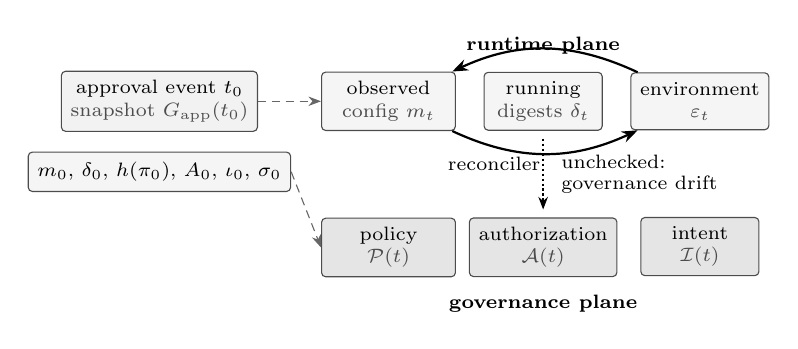
\begin{tikzpicture}[node distance=3.2mm and 4mm]
  % approval event
  \node[human, minimum width=20mm] (appr) at (0,0)
    {approval event $t_0$\\{\smlbl snapshot $\Gapp(t_0)$}};
  \node[attn, below=2.5mm of appr, minimum width=20mm] (snap)
    {$m_0$, $\delta_0$, $\dig(\pi_0)$, $A_0$, $\iota_0$, $\sigma_0$};

  % runtime plane
  \node[stage, right=8mm of appr, minimum width=17mm] (r1)
    {observed\\{\smlbl config $m_t$}};
  \node[stage, right=3.5mm of r1, minimum width=15mm] (r2)
    {running\\{\smlbl digests $\delta_t$}};
  \node[stage, right=3.5mm of r2, minimum width=15mm] (r3)
    {environment\\{\smlbl $\varepsilon_t$}};
  \node[lbl, above=1mm of r2] {\textbf{runtime plane}};
  \draw[flow] (r1) to[out=-25,in=205] node[lbl, below, pos=0.22]{reconciler} (r3);
  \draw[flow] (r3) to[out=155,in=25] (r1);

  % governance plane
  \node[evid, below=11mm of r1, minimum width=17mm] (g1)
    {policy\\{\smlbl $\Pol(t)$}};
  \node[evid, below=11mm of r2, minimum width=15mm] (g2)
    {authorization\\{\smlbl $\Auth(t)$}};
  \node[evid, below=11mm of r3, minimum width=15mm] (g3)
    {intent\\{\smlbl $\Int(t)$}};
  \node[lbl, below=1mm of g2] {\textbf{governance plane}};

  \draw[eflow] (appr.east) -- (r1.west);
  \draw[eflow] (snap.east) -- (g1.west);

  % the gap
  \draw[bflow] ($(r2.south)+(0,-1mm)$) -- node[lbl, right=1mm, text=black, align=left]
    {unchecked:\\governance drift} ($(g2.north)+(0,1mm)$);
\end{tikzpicture}
}
\caption{Approved intent versus runtime reality. The approval event at $t_0$
freezes a snapshot: configuration, policy version, authorization basis, intent
linkage, and environment assumptions. Afterward, two planes evolve
independently: the runtime plane (observed configuration, running artifacts,
environment) and the governance plane (policy versions, authorization
validity, intent records). Reconcilers continuously compare within the runtime
plane (solid loop); nothing in standard practice compares the runtime plane
against the \emph{evolved} governance plane (dashed gap)---the space in which
governance drift lives.}
\label{fig:planes}
\end{figure}

We fix vocabulary relative to an \emph{approval event}: the moment a change
was legitimized for an environment. \Cref{fig:planes} shows the two planes
that subsequently evolve. All definitions are made precise in the model of
\cref{sec:model}; here we give their content and their separations.

\begin{definition}[Approved State]
\label{def:approved}
The \emph{approved state} of a deployment is an append-only sequence of
immutable snapshots, one per approval event. Each snapshot records: the
approved configuration (manifest content and the
artifact digests it resolves to), the policy version under which it was
evaluated, immutable authorization proof (approvals, exceptions, their
subjects, scopes, execution times, and windows), the intent linkage (the change record and revision the
approval covers), and the declared environment assumptions within which the
risk assessment was made. Evaluation selects the latest applicable covering
snapshot; prior snapshots remain evidence rather than being overwritten.
\end{definition}

\begin{definition}[Configuration Drift]
\label{def:confdrift}
Divergence between the \emph{current desired} configuration and the
\emph{observed} configuration: $\Gobs(t) \ne$ desired$(t)$. This is the
classical notion~\cite{awsconfig,driftctl,nist800128}, decidable by
comparison of present states.
It is an operational component of the umbrella vector; by itself it does not
assert that either state is unauthorized.
\end{definition}

\begin{definition}[Policy Drift]
\label{def:poldrift}
Divergence between the policy version $\pi_B$ pinned in the selected admitted
basis $B_x(t)$ and the policy
context now governing the environment, \emph{as it bears on this deployment}:
$\Pol(t)$ has changed such that the running configuration would not be
admitted under it today, although it was compliant when approved.
\end{definition}

\begin{definition}[Authorization Drift]
\label{def:authdrift}
Invalidation or mismatch of the authorization basis without any configuration
event: a continuing approval or temporary exception lapsed while its effect
persists; an applicable approval was revoked under its declared prospective
or retroactive semantics; or the running artifact's digest is not the subject
any valid approval refers to. A one-shot approval need only have been valid at
execution, provided its integrity-valid proof survives.
\end{definition}

\begin{definition}[Intent Drift]
\label{def:intdrift}
Divergence between the content now driving the runtime and the intent record
the authorization covers: the desired state was changed (e.g., rolled back)
to content whose approval basis is absent or belongs to a different change,
and reconciliation faithfully executes it.
\end{definition}

\begin{definition}[Evidence Drift]
\label{def:evddrift}
Decay of the records connecting the running state to its approval basis: the
chain (revision $\to$ artifact $\to$ deployment $\to$ approval) can no longer
be established from surviving evidence, so governance consistency becomes
\emph{undecidable} rather than false. Evidence drift converts governance
questions from answerable to unanswerable. It is therefore an
\emph{epistemic, transversal} class: unlike the five substantive components,
it does not assert that a governed relation is inconsistent; it records that
one or more such relations can no longer be decided. We keep it inside the
governance-drift umbrella because the operational response---repair evidence
and withhold a polar verdict---is class-specific.
\end{definition}

\begin{definition}[Environment Drift]
\label{def:envdrift}
Violation, outside the managed configuration's scope, of an environment
predicate recorded by the approval's risk assessment: IAM scope broadened,
network exposure altered, an adjacent cloud resource modified out of
band---no desired state exists for the changed property, so no
configuration comparison can even represent the divergence.
\end{definition}

\begin{definition}[Governance Drift]
\label{def:govdrift}
The condition in which the operational state of an environment diverges from
the state, policy context, authorization basis, intent, or environment
assumptions under which it was approved, together with the epistemic condition
in which one or more such relations can no longer be decided. Formally, the
umbrella contains five substantive divergence components
(\cref{def:confdrift,def:poldrift,def:authdrift,def:intdrift,def:envdrift})
and one transversal evidence condition (\cref{def:evddrift}). A deployment is
\emph{governance-consistent} at $t$ when every substantive divergence of
\cref{sec:model} is zero and every required component is decidable. The
substantive components are not mutually exclusive: one incident may
drift several at once (an unapproved rollback drifts intent \emph{and}
leaves the runtime on digests no valid approval covers), which is one reason
the model of \cref{sec:model} keeps them as a vector.
\end{definition}

\subsection{Risk Channels and Severity}
\label{sec:severity}

The five substantive divergence components and the epistemic evidence class
are \emph{not} equivalent in ontology or consequence. A raw count
therefore cannot stand in for severity. Each class opens a different primary
risk channel and implies a different default disposition, as summarized in
\cref{tab:severity}. Configuration drift first threatens operational
integrity; policy drift threatens compliance with the currently governing
control; authorization drift threatens security legitimacy; intent drift
threatens the legitimacy of the change itself; evidence drift threatens audit
and forensic decidability; and environment drift changes the exposure or
assumption boundary around the approved system.

\begin{table*}[t]
\centering
\caption{Proposed Class-Resolved Risk Channels and Illustrative Default
Response Families. These Rows Are Not Empirically Validated or a Scalar
Ranking: Actual Severity Depends on Blast Radius, Exposure Duration,
Reversibility, Consequence, and Evidence Coverage.}
\label{tab:severity}
\footnotesize
\begin{tabular}{@{}p{0.14\textwidth}p{0.23\textwidth}p{0.28\textwidth}p{0.25\textwidth}@{}}
\toprule
Drift class & Primary risk channel & Governance question & Default response family \\
\midrule
Configuration & Operational availability and integrity & Does observed state still match the managed desired state? & Reconcile, contain, or accept an explicit runtime exception \\
Policy & Compliance and control validity & Would the running state satisfy the policy governing it now? & Re-evaluate, migrate under an SLA, or document a current exception \\
Authorization & Security and privilege legitimacy & Is the running subject still covered by valid authority? & Revoke, block, contain, or page the accountable owner \\
Intent & Governance and change legitimacy & Does the deployed revision implement the change that was approved? & Halt propagation, restore the authorized revision, or obtain new approval \\
Evidence & Audit and forensic decidability & Can the approval basis and lineage still be established? & Preserve records, escalate, and report \emph{undecidable} rather than compliant \\
Environment & Assumption and exposure boundary & Do unmanaged surroundings still satisfy the recorded risk assumptions? & Contain exposure and reassess the approval in the changed environment \\
\bottomrule
\end{tabular}
\end{table*}

This mapping is causal, not ordinal: drift class $\rightarrow$ risk channel
$\rightarrow$ response family. Within a class, severity must still be
conditioned on asset criticality, affected subjects, exposure time,
reversibility, and the confidence permitted by surviving evidence. Across
classes, a low-impact authorization mismatch can be less severe than a
configuration fault that stops a safety-critical service. The taxonomy thus
supports class-specific prioritization without pretending that one universal
weight orders every incident.

\begin{figure}[t]
\centering
\resizebox{\columnwidth}{!}{% Drift taxonomy (single column, resized)
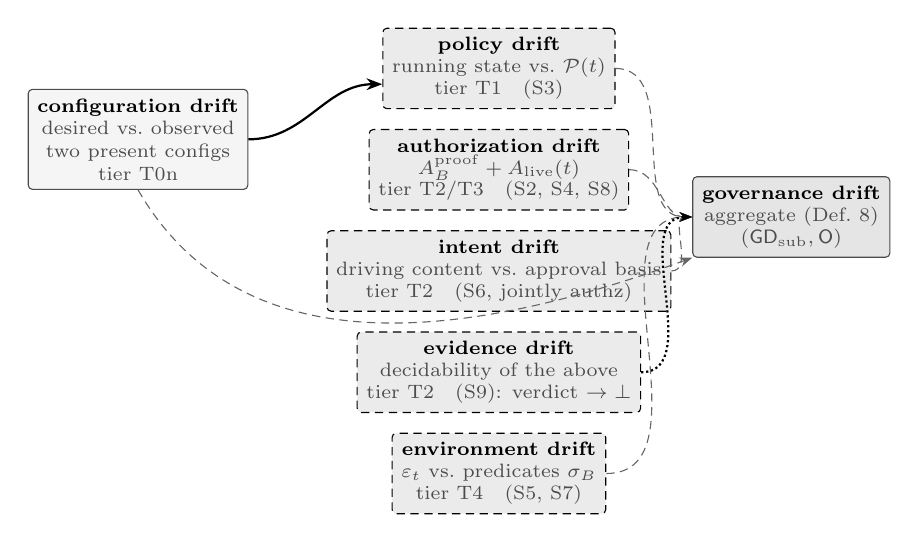
\begin{tikzpicture}[node distance=2.8mm and 3mm]
  \node[stage, minimum width=24mm] (conf) at (0,0)
    {\textbf{configuration drift}\\{\smlbl desired vs.\ observed}\\{\smlbl two present configs}\\{\smlbl tier T0n}};
  \node[brok, right=17mm of conf, minimum width=27mm, yshift=9mm] (pol)
    {\textbf{policy drift}\\{\smlbl running state vs.\ $\Pol(t)$}\\{\smlbl tier T1 \; (S3)}};
  \node[brok, below=2.5mm of pol, minimum width=27mm] (auth)
    {\textbf{authorization drift}\\{\smlbl $A_B^{\rm proof}+A_{\rm live}(t)$}\\{\smlbl tier T2/T3 \; (S2, S4, S8)}};
  \node[brok, below=2.5mm of auth, minimum width=27mm] (int)
    {\textbf{intent drift}\\{\smlbl driving content vs.\ approval basis}\\{\smlbl tier T2 \; (S6, jointly authz)}};
  \node[brok, below=2.5mm of int, minimum width=27mm] (evd)
    {\textbf{evidence drift}\\{\smlbl decidability of the above}\\{\smlbl tier T2 \; (S9): verdict $\to \unk$}};
  \node[brok, below=2.5mm of evd, minimum width=27mm] (env)
    {\textbf{environment drift}\\{\smlbl $\varepsilon_t$ vs.\ predicates $\sigma_B$}\\{\smlbl tier T4 \; (S5, S7)}};

  \node[evid, right=8mm of auth.east, minimum width=20mm, yshift=-6mm] (gov)
    {\textbf{governance drift}\\{\smlbl aggregate (Def.~8)}\\{\smlbl $(\GDsub,\ObsMask)$}};

  \draw[flow] (conf.east) to[out=0,in=180] ($(pol.west)+(0,-2mm)$);
  \foreach \n in {pol,auth,int,env}
    \draw[eflow] (\n.east) to[out=0,in=180] (gov.west);
  \draw[bflow] (evd.east) to[out=0,in=180] (gov.west);
  \draw[eflow] (conf.south) to[out=-60,in=200] (gov.south west);
\end{tikzpicture}
}
\caption{The drift taxonomy. Configuration drift (left) is a relation between
two present configurations. Five substantive components relate the present
state to the approved snapshot or evolved context; evidence drift is the
transversal loss of decidability shown by the dotted path. Their umbrella is
governance drift (\cref{def:govdrift}). Annotated
under each class: the evidence tier of \cref{sec:architecture} that first
decides it, as measured in \cref{sec:study}.}
\label{fig:taxonomy}
\end{figure}

\subsection{The Central Separation}
\label{sec:separation}

The taxonomy's load-bearing claim is that \cref{def:govdrift} does not reduce
to \cref{def:confdrift}. We establish it constructively and then in general
form.

\subsubsection{Constructed counterexamples}
\Cref{fig:example} presents the canonical scenario in full: a deployment
whose observed configuration equals its desired configuration at every instant
shown, and which passes from governance-consistent to governance-inconsistent
three separate times---at the policy supersession (policy drift), at the
exception expiry (authorization drift), and at the registry re-tag
(authorization drift at digest granularity). In the fourth panel the desired
state itself is rolled back and the reconciler \emph{eliminates} the
transient configuration drift by converging to content with no valid approval
basis: reconciliation manufactures intent drift while restoring configuration
consistency. Each panel is realizable with standard tooling, and each is one
of the executed scenarios of \cref{sec:study}.

\begin{figure*}[t]
\centering
\resizebox{\textwidth}{!}{% Config-consistent but governance-inconsistent: four-panel timeline (two-column)
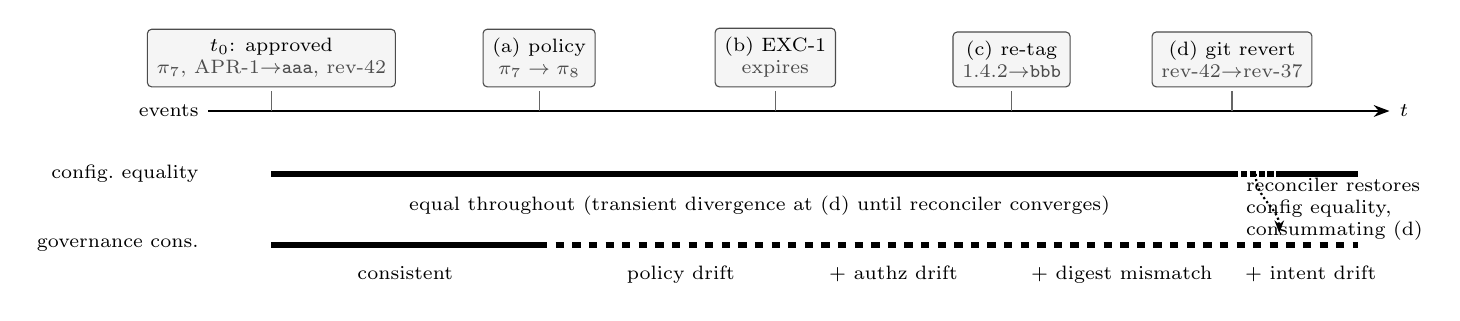
\begin{tikzpicture}[x=1mm, y=1mm]
  % timeline base
  \def\W{150}
  \draw[flow] (0,0) -- (\W,0) node[lbl, right]{$t$};
  \node[lbl, left] at (0,0) {events};

  % event marks
  \foreach \x/\lab in {8/{$t_0$: approved\\{\smlbl $\pi_7$, APR-1$\to$\texttt{aaa}, rev-42}},
                       42/{(a) policy\\{\smlbl $\pi_7 \to \pi_8$}},
                       72/{(b) EXC-1\\{\smlbl expires}},
                       102/{(c) re-tag\\{\smlbl 1.4.2$\to$\texttt{bbb}}},
                       130/{(d) git revert\\{\smlbl rev-42$\to$rev-37}}}{
    \draw[black!60] (\x,0) -- (\x,2.5);
    \node[attn, above=0mm] at (\x,3) {\lab};
  }

  % configuration-consistency band
  \node[lbl, left] at (0,-8) {config.\ equality};
  \draw[line width=2.2pt, black] (8,-8) -- (130,-8);
  \draw[line width=2.2pt, black, densely dotted] (130,-8) -- (136,-8);
  \draw[line width=2.2pt, black] (136,-8) -- (\W-4,-8);
  \node[lbl, below] at (70,-9.5) {equal throughout (transient divergence at (d) until reconciler converges)};

  % governance-consistency band
  \node[lbl, left] at (0,-17) {governance cons.};
  \draw[line width=2.2pt, black] (8,-17) -- (42,-17);
  \draw[line width=2.2pt, black, dashed] (42,-17) -- (\W-4,-17);
  \node[lbl, below] at (25,-18.5) {consistent};
  \node[lbl, below] at (60,-18.5) {policy drift};
  \node[lbl, below] at (87,-18.5) {$+$ authz drift};
  \node[lbl, below] at (116,-18.5) {$+$ digest mismatch};
  \node[lbl, below] at (140,-18.5) {$+$ intent drift};

  % reconciler annotation at (d)
  \draw[bflow] (133,-8) to[out=-90,in=90] (136,-15.5);
  \node[lbl, text=black, align=left] at (143,-12.5)
    {reconciler restores\\config equality,\\consummating (d)};
\end{tikzpicture}
}
\caption{Configuration-consistent but governance-inconsistent, in four
panels. Timeline of one deployment: observed configuration (bottom band)
remains equal to desired configuration throughout---configuration drift is
zero at every instant after reconciliation---while governance consistency
(top band) is broken successively by (a)~policy supersession
$\pi_7 \to \pi_8$, (b)~expiry of emergency exception \textsc{exc-1} whose
effect persists, (c)~registry re-tag moving \texttt{svc:1.4.2} to a digest no
approval references, and (d)~a Git rollback that the reconciler faithfully
converges to, eliminating transient configuration drift while stranding the
runtime on content whose approval belongs to a different change. Panels
correspond to Scenarios S3, S2, S4, and S6 of \cref{sec:study}.}
\label{fig:example}
\end{figure*}

\subsubsection{The dependency form}
\begin{proposition}[Configuration equality does not decide governance
consistency]
\label{prop:impossible}
Let $D$ be any detector whose inputs are configuration pairs
$(\mathit{desired}(t), \Gobs(t))$---including their full histories. There
exist worlds $w_1, w_2$ with identical configuration-pair histories in which
the same deployment is governance-consistent in $w_1$ and
governance-inconsistent in $w_2$. Hence no such $D$ decides governance
consistency, for any diffing sophistication.
\end{proposition}
\begin{proof}
Take $w_1$ and $w_2$ to agree on all configurations at all times and differ
only in the governance plane: in $w_2$ the policy version governing the
environment was superseded after $t_0$ by one the running configuration
violates (or: an exception's window elapsed; or: a valid approval in $w_1$ is
absent in $w_2$ for the same content). These differences live in
$\Pol(t), \Auth(t), \Int(t)$, which are not functions of the configuration
pair; both worlds present $D$ with identical inputs, and
\cref{def:govdrift} assigns them different values. $D$ outputs the same answer
in both, so it errs in one.
\end{proof}

The proposition is elementary---a definitional-dependency observation, and
we bill it as such rather than as a deep impossibility theorem. Its force is
architectural: it says deployed drift detectors are not approximations of
governance-drift detectors but detectors \emph{of a different relation}, and
no incremental improvement of configuration diffing closes the gap
\emph{as a decision procedure}. Two bounds on what it claims: it rules out
\emph{deciding}, not statistical \emph{hinting}---in real estates,
governance-plane events often correlate with configuration-plane events
(policy revisions ship alongside config pushes; rollbacks are visible in Git
history), so configuration histories may carry probabilistic signal about
governance state; how much is an empirical question for the laboratory, which
our closed world deliberately does not answer. And it says nothing against
comparison as a \emph{mechanism}: the governance tiers of
\cref{sec:architecture} are themselves comparisons---against recorded
bases, validity clocks, and coverage sets---which is precisely the point:
the input vocabulary, not the mechanism, is what must widen.

\subsubsection{What configuration drift remains}
The separation does not demote configuration drift: unauthorized manual
change (\cref{sec:study}, S1) is both configuration and governance drift, and
configuration comparison is its right detector. The taxonomy's point is
containment, not replacement: configuration drift is one of five substantive
components under the six-class umbrella, and the only one decidable in the
configuration vocabulary---which the study confirms
empirically as a detectability staircase whose first step is exactly that one
class.

\section{A Formal Model of Governance Drift (RQ2, RQ4)}
\label{sec:model}

\subsection{States and Contexts}
\label{sec:model-states}

Fix a deployment $x$ into environment $e$ with approval events at
$t_0<\cdots<t_k\leq t$.

\textbf{Approved-snapshot history.} Per \cref{def:approved}, every approval
event appends an immutable snapshot
\[
\begin{aligned}
\Gapp^{x}(t)&=\{G_{\mathrm{app}}^{(0)}(t_0),\ldots,
G_{\mathrm{app}}^{(k)}(t_k)\},\\
G_{\mathrm{app}}^{(i)}&=\bigl(m_i,\delta_i,\dig(\pi_i),A_i^{\mathrm{proof}},
\iota_i,\sigma_i\bigr).
\end{aligned}
\]
Each record contains the approved manifest content $m_i$ and artifact digests $\delta_i$ it
resolved to at approval; the pinned policy version; the authorization basis
$A_i^{\mathrm{proof}}$ (the immutable proof that approval instruments covered
the named subjects and scope at their execution times); the intent linkage $\iota_i$ (change
record, revision); and the environment assumptions $\sigma_i$ (the declared
properties of $e$---identity scopes, exposure---under which risk was
assessed). Let $b(t)$ select the greatest $i$ such that $t_i\leq t$ and the
snapshot scope covers $(x,e)$. The admitted basis is
\[
B_x(t)=G_{\mathrm{app}}^{(b(t))}
=\bigl(m_B,\delta_B,\dig(\pi_B),A_B^{\mathrm{proof}},
\iota_B,\sigma_B\bigr).
\]
Selection does not require current validity: an expired or revoked basis must
remain selected so its divergence can be reported. Superseded snapshots
remain available for audit and lineage; benign reapproval appends a new basis
rather than mutating history. Append-only means records cannot be rewritten,
not that their storage cannot be lost; loss of $A_B^{\mathrm{proof}}$ is an
evidence failure, as S9 exercises.

\textbf{Observed state.} $\Gobs(t) = (m_t, \delta_t, \varepsilon_t)$: the
observed configuration, the digests actually executing, and the observed
environment properties needed to evaluate the predicates in $\sigma_B$.

\textbf{Contexts.} Three time-indexed context streams:
$\Pol(t)$, the policy version(s) governing $e$ at $t$ with their evaluation
semantics; $\Auth_{\mathrm{live}}(t)$, the authenticated current administrative
state of instruments (revocations, continuing validity, expiry); and $\Int(t)$, the intent records and the
desired-state revision currently driving delivery. Evidence availability,
where needed, is a fourth stream $\Evd(t)$ (the records from which the above
can be established).

\textbf{Authorization semantics.} Every instrument $a$ declares
$\mathrm{mode}(a)\in\{\text{one-shot},\text{continuing},
\text{temporary-exception}\}$, subject, scope, validity interval, and
revocation policy. One-shot authority is required at execution and its proof
is retained afterward; continuing authority must remain valid while its
effect persists; a temporary exception is continuing only until its expiry.
Revocation is prospective unless the record explicitly declares retroactive
invalidation. Let $\mathrm{NeedsLive}(a)$ hold for continuing and temporary
instruments, and for a one-shot instrument only when its declared revocation
policy permits retroactive invalidation. For an effect executed at $\tau$,
let $\mathrm{AppObs}(a,t)$ mean that its proof is available and, whenever
$\mathrm{NeedsLive}(a)$ holds, authenticated live status is also available.
Write $V_1$ for validity at $\tau$ without retroactive revocation, $V_c$
for current validity without revocation, and $V_e$ for $V_c$ while the
declared exception has not expired. Define the three-valued applicability function
\[
\mathrm{Applicable}(a,\tau,t)=
\begin{cases}
\bot,&\neg\mathrm{AppObs}(a,t);\\
V_1(a,\tau,t),&\text{one-shot};\\
V_c(a,t),&\text{continuing};\\
V_e(a,t),&\text{temporary exception}.
\end{cases}
\]
A retained historical proof is therefore not confused with currently
effective authority. Missing proof or live status yields undecidable where
the selected mode requires it; an authenticated revocation yields a polar
inconsistent verdict.

\textbf{Legitimate successors.} Let
$\mathrm{Succ}(\iota_B,t)$ be the set of revisions $\iota_n$ for which
there exists a finite chain $\iota_B,\iota_1,\ldots,\iota_n$ with transition
execution times $\tau_1,\ldots,\tau_n$, such that every edge
$(\iota_{j-1},\iota_j)$ and its artifact digest are covered by an instrument
$a_j$ for which $\mathrm{Applicable}(a_j,\tau_j,t)$ holds. A revision is a
legitimate successor iff it belongs to this set.
This definition excludes mere Git ancestry: lineage without a valid approval
edge does not extend the admitted basis.

\subsection{The Governance-Divergence Vector}
\label{sec:model-distance}

We define one divergence component per substantive relation; each is a function of exactly the
inputs its component needs, which is what makes the detectability results of
\cref{sec:study} possible to state.

\begin{itemize}[leftmargin=1.5em,itemsep=1.5pt,topsep=2pt]
\item $\dconf(t)$: a normalized difference over the managed configuration
graph between desired$(t)$ and $m_t$ (field-level graph diff with
runtime-owned fields factored out; \cref{sec:study} shows the normalization
is not cosmetic but the difference between signal and noise). This is an
operational consistency component included to give the evaluator a complete
control-state report; nonzero $\dconf$ alone does not imply that either the
desired or observed state lacks authorization coverage.
\item $\dpol(t)$: the set of controls in $\Pol(t)$ that the running state
violates although $B_x(t)$ records compliance under $\pi_B$---empty iff admission would
re-succeed under today's policy. Reported as a violated-control set, not a
number: policy versions form a revision structure, not a metric space, and
``how far'' is policy-weighted judgment, not geometry.
\item $\dauth(t)$: the set of relied-upon instruments for which
$\mathrm{Applicable}(a,\tau,t)$ is false, plus running digests in $\delta_t$
not covered by an applicable instrument grounded in $A_B^{\mathrm{proof}}$
and $\Auth_{\mathrm{live}}(t)$. If applicability is $\bot$, the authorization
mask entry is zero and the substantive component is undecidable rather than
included in this set.
\item $\dint(t)$: the mismatch between the revision driving delivery and the
revision the valid authorization covers: the current revision is outside
$\{\iota_B\}\cup\mathrm{Succ}(\iota_B,t)$.
\item $\denv(t)=\{q\in\sigma_B:q(\varepsilon_t)=\mathrm{false}\}$. The laboratory's
declared IAM-scope and exposure fields instantiate equality predicates, but
the definition permits ranges, membership, and monotone safety predicates.
\end{itemize}

Evidence availability is ontologically different from those distances. Define
the observability mask
$\ObsMask(t)=(o_{\mathrm{conf}},o_{\mathrm{pol}},o_{\mathrm{auth}},
o_{\mathrm{int}},o_{\mathrm{env}})$, where $o_j=1$ iff every required item in
the component's evidence contract is present, complete, fresh within its
declared bound, integrity-valid, source-authenticated, linked to subject
$x$, and delivered by a healthy stream. Confidence is therefore not an
unscoped probability: it is a named contract and threshold published with
the evaluator. A missing or contract-failing record yields \emph{undecidable};
an authenticated record stating ``revoked,'' ``negative,'' or ``never
issued'' is available evidence and may yield \emph{inconsistent}. Evidence drift is a
transition of any required $o_j$ from one to zero. Each substantive component
therefore has three-valued reporting semantics---consistent, inconsistent, or
undecidable---but only the first two are values of the substantive relation.

\begin{definition}[Governance Divergence Vector; Consistency]
\label{def:gd}
$\GDsub(t) = \bigl(\dconf, \dpol, \dauth, \dint, \denv\bigr)(t)$ and
$\GD(t)=(\GDsub(t),\ObsMask(t))$. Operational consistency
$\mathsf{OpCons}(x,t)$ holds iff $\dconf=0$ and its evidence is decidable.
Governance coverage $\mathsf{GovCov}(x,t)$ holds iff
$\dpol=\dauth=\dint=\denv=0$ and their mask entries are one. Total
$\Cons(x,t)=\mathsf{OpCons}(x,t)\land\mathsf{GovCov}(x,t)$. Onset of governance drift is
$\inf\{t > t_0 : \lnot\Cons(x,t)\}$; \emph{dwell time} is the duration of
inconsistency; \emph{detection latency} is detection time minus onset.
\end{definition}

\begin{figure}[t]
\centering
\resizebox{\columnwidth}{!}{% Drift lifecycle timeline (single column, resized)
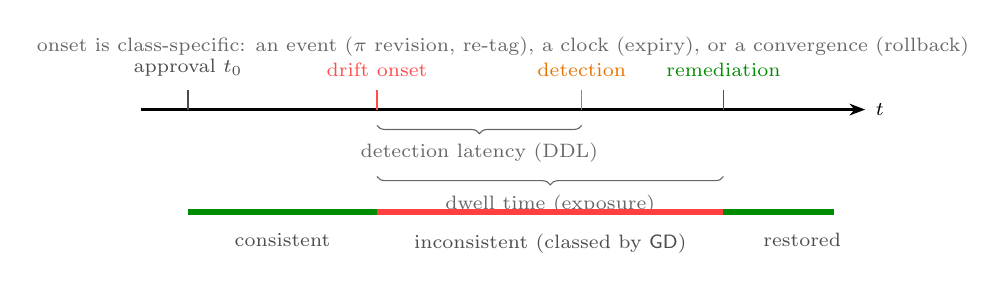
\begin{tikzpicture}[x=1mm, y=1mm]
  \def\W{92}
  \draw[flow] (0,0) -- (\W,0) node[lbl, right]{$t$};
  \foreach \x/\lab/\col in {6/{approval $t_0$}/black!70,
                            30/{drift onset}/red!70,
                            56/{detection}/orange!90!black,
                            74/{remediation}/green!55!black}{
    \draw[\col] (\x,0) -- (\x,2.5);
    \node[lbl, above, text=\col] at (\x,3) {\lab};
  }
  \draw[decorate,decoration={brace,mirror,amplitude=3pt}, black!60]
    (30,-2) -- (56,-2) node[midway, below=3pt, lbl] {detection latency (DDL)};
  \draw[decorate,decoration={brace,mirror,amplitude=3pt}, black!60]
    (30,-8.5) -- (74,-8.5) node[midway, below=3pt, lbl] {dwell time (exposure)};
  \node[lbl, below=1mm] at (18,-13.5) {\smlbl consistent};
  \draw[line width=2.2pt, green!55!black] (6,-13) -- (30,-13);
  \draw[line width=2.2pt, red!75] (30,-13) -- (74,-13);
  \draw[line width=2.2pt, green!55!black] (74,-13) -- (\W-4,-13);
  \node[lbl, below=1mm, text=red!75] at (52,-13.5) {\smlbl inconsistent (classed by $\GD$)};
  \node[lbl, below=1mm] at (84,-13.5) {\smlbl restored};
  \node[lbl, text=black!60] at (46,8)
    {onset is class-specific: an event ($\pi$ revision, re-tag), a clock (expiry), or a convergence (rollback)};
\end{tikzpicture}
}
\caption{The drift lifecycle and its temporal quantities
(\cref{def:gd}). Onset is class-specific---an organizational event (policy
revision), a clock crossing (exception expiry), an exogenous event
(registry re-tag), or a reconciler convergence (rollback). Detection latency
is the tier-dependent quantity measured in \cref{sec:study}; dwell time is
the exposure window that remediation closes, with the remediation family
determined by the drifted component (\cref{sec:model-vector}).}
\label{fig:lifecycle}
\end{figure}

\subsection{Why the Distance Is a Vector, Not a Scalar}
\label{sec:model-vector}

A scalar $\GD$ was the natural first proposal, and we reject it as primitive
for three reasons. \emph{Incommensurability}: the components take values in
different structures (graph diffs, control sets, validity states,
three-valued verdicts); any scalarization imports policy weights, and those
weights are governance choices, not properties of the system.
\emph{Remediation asymmetry}: the components have different remediations---%
reconcile ($\dconf$), re-evaluate and re-approve or migrate ($\dpol$),
re-authorize or terminate the exception ($\dauth$), restore or re-approve
intent ($\dint$), restore assumptions or re-assess ($\denv$), repair evidence
where $\ObsMask$ is zero---so collapsing them destroys exactly the information an operator
needs. \emph{Temporal structure}: components drift on different clocks
(policy revisions are discrete organizational events; exception expiry is a
scheduled instant; registry re-tags are exogenous), so a scalar time series
conflates processes that must be attributed separately. A weighted composite
for reporting is legitimate \emph{on top of} the vector (\cref{sec:metrics}),
with published weights, exactly as a risk score summarizes but does not
replace findings.

\subsection{Detectability, Formally}
\label{sec:model-detect}

Each component divergence is a function of specific streams:
$\dconf$ of (desired, $\Gobs$); $\dpol$ additionally of $\Pol(t)$ and
$\pi_B$; $\dauth$ of $A_B^{\mathrm{proof}}$, $\Auth_{\mathrm{live}}(t)$,
execution times, and $\delta_t$; $\dint$ of $\Int(t)$ and $\iota_B$;
$\denv$ of $\varepsilon_t$ and $\sigma_B$; and every
entry of $\ObsMask$ of the evidence needed for its corresponding computation.
\Cref{prop:impossible} is the negative direction of this
dependency structure; the positive direction is equally direct:

\begin{proposition}[Tier sufficiency]
\label{prop:tiers}
A detector with access to the streams a component depends on decides that
component's consistency (in the closed-world model, exactly; in the field, up
to the fidelity of the streams). Consequently a sufficient detector for full
governance consistency joins the configuration comparison with the policy,
authorization, intent/lineage, and environment streams---the tiered
architecture of \cref{sec:architecture}, whose scenario-to-tier realization
\cref{sec:study} checks cell by cell.
\end{proposition}
\begin{proof}
Each component divergence in \cref{sec:model-distance} is defined as a
computable function of the named streams; providing the streams provides the
function's inputs.
\end{proof}

The proposition is an input-enumeration result; whether a concrete
implementation realizes it is a separate, checkable question---%
\cref{sec:study} performs exactly that check on our released reference
semantics, and \emph{only} that check: agreement there validates the
implementation, not the model.

\begin{proposition}[Tier minimality]
\label{prop:tier-minimality}
For every stream added at T1--T4, there exist two worlds that are
indistinguishable to every lower tier but have different governance verdicts
for a component first decidable from that stream. Therefore no lower tier
decides that component in general.
\end{proposition}
\begin{proof}
Construct the pairs while holding all lower-tier observations fixed. For T1,
keep desired and observed configuration identical and let the current policy
admit the deployment in one world but reject it in the other. For T2, keep the
T1 projection fixed and let the same effective exception be valid in one world
but expired in the other; alternatively, retain versus delete its approval
record, changing the authorization/intent mask from decidable to undecidable.
For T3, keep the manifest tag and every T2 stream fixed but let the running tag
resolve to an approved digest in one world and an uncovered digest in the
other. For T4, keep all T3 streams fixed and change only an unmanaged
environment property recorded in $\sigma_B$. Each pair has identical
lower-tier projections and different component verdicts, so any lower-tier
detector returns the same value in both and errs in one.
\end{proof}

Unlike \cref{prop:tiers}, this is a necessity result: the staircase is not
merely a convenient implementation decomposition. Its scope remains relative
to the declared component semantics; adding a genuinely equivalent stream at
a lower tier widens that tier's projection rather than refuting the result.

Two modeling notes bound the claims. First, \emph{granularity}: whether the
registry re-tag scenario is ``configuration'' drift depends on reference
semantics---under tag semantics the configuration is unchanged; under digest
semantics it changed. The model takes no side: it requires only that
$B_x(t)$ record resolved digests, which relocates the question from metaphysics
to evidence (what did the approval bind?), where \cref{sec:study} shows it is
decidable at the lineage tier. Second, \emph{legitimate context change}:
policy supersession does not make drift \emph{culpable}---the deployment was
legitimate under $\pi_7$ and the organization changed the rules. The model
deliberately measures divergence, not blame; whether policy drift triggers
migration, exemption, or re-approval is a governance decision the vector
informs (\cref{sec:discussion}).

\section{A Tiered Detection Architecture}
\label{sec:architecture}

\Cref{prop:impossible,prop:tiers} together prescribe the architecture:
governance-drift detection is configuration comparison \emph{plus} the
minimal additional evidence streams, joined against the selected admitted basis.
\Cref{fig:architecture} organizes it as cumulative tiers, each named for what
it adds and each mapped to the drift classes it first decides.

\begin{figure*}[t]
\centering
\resizebox{0.93\textwidth}{!}{% Tiered detection architecture (single column, resized)
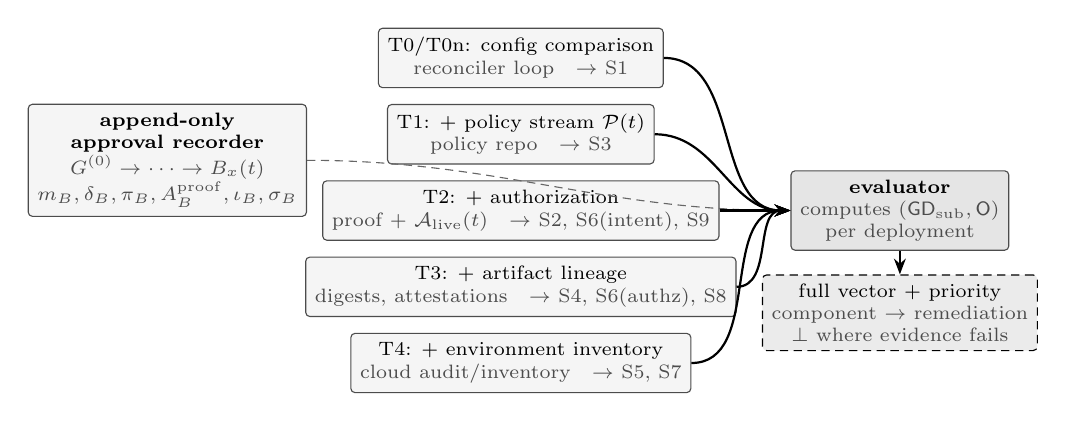
\begin{tikzpicture}[node distance=2.6mm and 4mm]
  \node[attn, minimum width=25mm] (snap) at (0,0)
    {\textbf{append-only}\\\textbf{approval recorder}\\{\smlbl $G^{(0)}\to\cdots\to B_x(t)$}\\{\smlbl $m_B,\delta_B,\pi_B,A_B^{\rm proof},\iota_B,\sigma_B$}};

  % tiers stack
  \node[stage, right=9mm of snap, minimum width=26mm, yshift=13mm] (t0)
    {T0/T0n: config comparison\\{\smlbl reconciler loop \; $\to$ S1}};
  \node[stage, below=2mm of t0, minimum width=26mm] (t1)
    {T1: $+$ policy stream $\Pol(t)$\\{\smlbl policy repo \; $\to$ S3}};
  \node[stage, below=2mm of t1, minimum width=26mm] (t2)
    {T2: $+$ authorization\\{\smlbl proof + $\Auth_{\rm live}(t)$ \; $\to$ S2, S6(intent), S9}};
  \node[stage, below=2mm of t2, minimum width=26mm] (t3)
    {T3: $+$ artifact lineage\\{\smlbl digests, attestations \; $\to$ S4, S6(authz), S8}};
  \node[stage, below=2mm of t3, minimum width=26mm] (t4)
    {T4: $+$ environment inventory\\{\smlbl cloud audit/inventory \; $\to$ S5, S7}};

  % evaluator
  \node[evid, right=9mm of t2, minimum width=22mm] (eval)
    {\textbf{evaluator}\\{\smlbl computes $(\GDsub,\ObsMask)$}\\{\smlbl per deployment}};
  \node[brok, below=3mm of eval, minimum width=22mm] (out)
    {full vector + priority\\{\smlbl component $\to$ remediation}\\{\smlbl $\unk$ where evidence fails}};

  \draw[eflow] (snap.east) to[out=0,in=180] (eval.west);
  \foreach \n in {t0,t1,t2,t3,t4}
    \draw[flow] (\n.east) to[out=0,in=180] (eval.west);
  \draw[flow] (eval) -- (out);
\end{tikzpicture}
}
\caption{Tiered governance-drift detection. The append-only recorder (left)
preserves successive approvals and selects $B_x(t)$. Evidence tiers (center) cumulatively widen
the detector's vocabulary: T0/T0n configuration comparison (the reconciler's
existing loop, naive or churn-normalized), T1 policy-version stream, T2
authorization records with validity semantics, T3 artifact lineage, T4
environment inventory. The evaluator (right) recomputes the component
divergences of \cref{sec:model-distance} continuously and emits classed drift
vectors plus an epistemic mask, with a priority projection and the remediation
family each component implies. Stream adapters also report the presence,
completeness, freshness, integrity, authenticity, subject linkage, and health
required by each component's evidence contract. Annotations show which components of
Scenarios S1--S9 each tier first detects, as measured in
\cref{sec:study}.}
\label{fig:architecture}
\end{figure*}

\subsection{Components}
\textbf{Approved-state recorder.} At approval, append an immutable pending
snapshot to $\Gapp^x$---manifest content, \emph{resolved} digests, policy-version pin,
immutable authorization proof with execution times, intent linkage, environment
assumptions, scope, and predecessor edge. At operational effect, append or
attest its activation; cancellation marks it aborted. Persist both events
durably and independently of the delivery
platforms. This is the architecture's one hard prerequisite: without a
recorded approval basis there is nothing to drift \emph{from}; where such
records are absent or decayed, the basis-dependent entries of
$\ObsMask_{\mu}(u,\theta;T)$ are zero and those components are undecidable. If
no independently evaluated component is known nonzero, the total status is
undecidable; if configuration or another independently established component
is known nonzero, the total status is inconsistent because known inconsistency
precedes unknown evidence. The desired/observed configuration component remains
comparable when its own evidence contract is satisfied; the evaluator must
report this partial vector and mask rather than either total consistency or
total ignorance.
Conflicting activated maxima also fail closed instead of being
ordered by approval timestamp (\cref{prop:basis-selection}).

\textbf{Evidence tiers.}
\emph{T0/T0n}: the desired/observed comparison every reconciler already
performs~\cite{argocd,fluxcd,awsconfig}; T0n normalizes runtime-owned fields
(replica counts under autoscaling, rollout hashes)---the study quantifies why
the naive form is unusable as a governance signal.
\emph{T1}: the policy-version stream from the policy engine's
repository~\cite{opa,kyverno}; the evaluator re-evaluates the running state
against $\Pol(t)$ and compares with the pinned basis.
\emph{T2}: authorization records with mode and validity semantics---expiry,
scope, prospective or retroactive revocation---bound to the expected change
graph, covered digests where the authorization scope requires them, and
immutable approval/exception proofs. Exceptions and approvals are therefore
evidenced objects with clocks, subjects, and coverage rather than booleans;
ITIL-style change records~\cite{itil4} and platform approvals both map here.
\emph{T3}: artifact lineage---digest-level linkage from running workloads to
approval subjects, the slice pioneered by supply-chain
attestation~\cite{slsa,torres2019,newman2022,binauthz}.
\emph{T4}: environment inventory---observation of the unmanaged properties
assumed at approval (IAM scope, exposure) and comparison against the
\emph{recorded} predicates $\sigma_B$ in $B_x(t)$, from cloud inventories,
audit streams, and telemetry correlation~\cite{cloudtrail,cspm,otel}.
Mechanically this is baseline comparison---CSPM's move---and we say so
plainly; the difference is the reference (the approval event's recorded
assumptions rather than a benchmark) and the joined, class-resolved verdict.

\textbf{Evaluator.} A continuous process (or scheduled sweep) computing
$\GD_{\mu}(u,\theta;T)$ per deployment: cheap incremental checks on context-change events
(policy revision published, exception clock elapsed, registry event), using
event-triggered recomputation where a source exposes deltas and scheduled or
background re-evaluation where it does not. Several scenarios
in \cref{sec:study} are detectable with zero latency at the tier that
carries the relevant modeled event; this is not a claim that live integrations
avoid polling or scans.

\textbf{Analytic scaling envelope.} For $n$ deployments with at most $m$
managed configuration fields, $r$ policy predicates, $a$ relied-upon
instruments, $d$ running digests, and $q$ environment predicates each, a full
sweep is $O(n(m+r+a+d+q))$ time. Retaining $s$ complete snapshots per
deployment costs $O(ns(m+a+d+q))$ storage, plus current-stream indices. The
intended execution is incremental: policy-to-deployment,
subject-to-approval, digest-to-workload, and predicate-to-resource indices
restrict an event to its $k$ affected deployments, yielding
$O(k(m+r+a+d+q))$ work. Policy results and immutable proofs are cacheable;
evaluators can shard by cluster, namespace, or tenant. Kubernetes watches and
batched cloud-inventory deltas avoid one API request per deployment. Cloud
quotas and cache invalidation remain engineering constraints. The in-memory
microbenchmark in \cref{tab:scaling} measures the join after decoding and
indexing inputs; it deliberately does not claim a Kubernetes or production
throughput bound.

\textbf{Minimal adoption path.} The smallest useful deployment is
T0n+T1+T2: normalize the reconciler comparison, re-evaluate running state
under current policy, and join durable approvals and exceptions with explicit
validity semantics. This separates operational, compliance, and authorization
risk immediately; T3 adds digest lineage and T4 adds declared environment
predicates as evidence maturity grows. Governance Conformance Coverage (GCC;
\cref{met:gcc}) is reported from the first rollout so unevaluable coverage is
visible rather than treated as conformance.

For legacy workloads, a discovery pass may create a signed
\emph{retrospective baseline} from current state, current policy results, and
an accountable owner's attestation. It is timestamped and labeled as
reconstructed evidence---never represented as a historical approval---and
GCC remains partial for facts that cannot be recovered. New changes then enter
the ordinary append-only path, allowing coverage to increase without
rewriting the estate's past.

\subsection{Threat and Trust Model}
The protected claim is integrity and decidability of the relation, not
availability of the workload. An attacker may mutate Git, tags, runtime
objects, policy results, authorization status, inventory, or one evidence
adapter; operators may also make the same changes accidentally. These sources
are therefore evidence inputs, not intrinsically trusted truth. The trusted
computing base (TCB) is the recorder/activation authority, stable-identity
issuer, authenticated time and adapter metadata, append-only log or external
anchor, basis selector, and evaluator code. Every record is subject-bound,
sequenced, freshness-bounded, and content-addressed; snapshots are complete
atomic tuples chained to their predecessors. A contract failure masks only
the dependent components and prevents a conformance claim.

A local hash chain detects modification and reordering of retained snapshots,
but cannot by itself prove that a privileged actor did not truncate the tail
or replace the entire history. Production deployment therefore requires an
external transparency anchor or threshold signatures, access separation, and
key/clock rotation records. Compromise of the evaluator and all anchors, or
collusion of the recorder and activation authority, is outside the model.
Denial of evidence remains visible as reduced GCC/undecidable; remediation may
keep a critical workload available, but it must not relabel uncertainty as
conformance (\cref{sec:discussion}).

\subsection{Relation to Existing Mechanisms}
The architecture is deliberately assembled from streams that already exist in
mature platforms; its novelty is the \emph{join semantics} against a recorded
approval basis and the class-resolved verdict. Admission
control~\cite{k8sadmission,opa,kyverno} evaluates the same predicates once,
at entry; continuous-validation features~\cite{binauthz} re-evaluate the
artifact-policy slice; posture management~\cite{cspm} scans environment
configuration against benchmark policy without any approved-state reference.
Indeed, per-tier continuous detection largely \emph{exists} in cited
tooling, and the architecture credits it explicitly: Kyverno's background
scanning re-evaluates existing resources against current policy (our
T1)~\cite{kyverno}; configuration recorders track unmanaged resources
(much of T4)~\cite{awsconfig,cspm}; continuous validation re-checks
artifact policy (part of T3)~\cite{binauthz}. Among the mechanisms in the
bounded source set documented in \cref{sec:related}, none jointly provides all
of the following: every tier evaluated against the
\emph{admitted basis} $B_x(t)$, with mode-aware validity on the authorization
itself, and verdicts that distinguish ``violates policy'' from ``was never
approved'' from ``was admitted legitimately and the world moved''---the
distinctions that determine remediation (\cref{sec:model-vector}). The
contribution is the relation and its join semantics, not the comparison
machinery, and \cref{sec:related} restates novelty in exactly those terms.

\section{Executed Study: Detectability Across Evidence Tiers (RQ2--RQ4)}
\label{sec:study}

We now measure the taxonomy's detectability structure. The study is executed
and deterministically reproducible from the packaged source
($\approx$380 lines of dependency-free Python; the results table, including
its header, is generated programmatically by the same run). Its
epistemic scope is stated plainly: it is a \emph{closed-world evaluation of
detector semantics}---the world, its scenarios, and the detectors are all
models---so it establishes what each evidence tier can and cannot decide
\emph{in principle}, with event-time latencies. It does not measure any real
cluster; wall-clock behavior on real infrastructure is the laboratory's job
(\cref{sec:lab}).

\subsection{Modeled World and Scenarios}
The world models one deployment with the selected admitted basis of
\cref{sec:model-states}---including recorded environment assumptions
$\sigma_B$---and streams for desired state (Git), observed cluster state,
registry contents, policy versions \emph{with evaluable requirement sets}
(so that T1 implements \cref{def:poldrift}'s admission re-evaluation, not a
version-string comparison), authorization records as a set with subject
digests, covered revisions, windows, and revocation (so that legitimate
successors are modeled), and two unmanaged environment properties. Each run
is 400 events; drift is injected at event 150. Twelve scenarios follow the
taxonomy and the constructed examples of \cref{fig:example}:

\begin{description}[leftmargin=2.6em,itemsep=1pt,topsep=2pt]
\item[S1] manual in-cluster change (observed field diverges from desired);
\item[S2] expired emergency authorization (exception granted with a 40-event
window; nothing removes it at expiry);
\item[S3] policy version change post-deploy ($\pi_7 \to \pi_8$, which the
running configuration violates);
\item[S4] artifact substitution (same tag re-pointed to a new digest,
rolled onto nodes; manifests unchanged);
\item[S5] IAM permission expansion out of band (unmanaged);
\item[S6] Git rollback without new approval (reconciler converges to the
reverted content; approval binds the newer revision);
\item[S7] out-of-band cloud console modification (unmanaged);
\item[S8] approval mismatch (deployed digest is not any approval's subject);
\item[S9] live-status deletion for a continuing approval: immutable
$A_B^{\mathrm{proof}}$ survives, but the authenticated source required to
establish continuing validity is lost; authorization and intent become
undecidable---the missing status is neither a revocation nor proof that approval never existed
(evidence drift---\cref{def:evddrift}---exercised directly);
\item[S10] policy supersession plus an expired exception
($\{\text{policy},\text{authorization}\}$);
\item[S11] artifact substitution plus environment change
($\{\text{authorization},\text{environment}\}$);
\item[S12] rollback plus deletion of its approval basis: the underlying
intent/authorization relations become undecidable, so the honest observable
output is evidence drift rather than a guessed polar set;
\end{description}
plus \textbf{S0}, a no-drift control. Churn is of two kinds, both present in
every stream including the control: \emph{runtime churn} (30\% of events:
autoscaler replica changes, rolling-restart hash changes) and \emph{benign
governance churn} (2\% of events: policy revisions the running state
satisfies, approved updates that legitimately advance revision, digest, and
approval together, and hygienic exceptions removed at expiry). The governance
churn exists so that the governance tiers' false-alarm rates are earned
against realistic governance noise rather than measured against a silent
plane.

\subsection{Detectors and Counterfactual Scoring}
Six detector tiers implement \cref{sec:architecture}: T0 (naive
configuration comparison, including runtime-owned fields), T0n (normalized),
and cumulative T1--T4, each a pure function of its tier's visible streams, so
tier capabilities are enforced by construction. Ground truth is a
\emph{class set} per scenario (components are a vector and may drift
together, \cref{def:govdrift}). The detector exports the complete class set
decidable at its tier; a priority-ordered first verdict is derived only as an
operational interface. We score exact-set agreement, subset-only partial
diagnosis, and Hamming loss rather than accepting any one member of the ground
truth. Missing approval records set the relevant entries of $\ObsMask$ to zero
and produce the explicit undecidable/evidence verdict, never a guessed polar
one. S6, S10, and S11 test substantive composition; S12 tests composition under
evidence loss.

Scoring required care, and the naive arm is why. A detector that alarms
constantly ``detects'' every scenario by coincidence; volume is not
information. We therefore score \emph{counterfactually}: for each (scenario,
tier, seed), the detector runs on the drift stream and on a paired,
same-seed, no-drift control stream with identical churn; the drift is
\emph{detected} iff the two alarm sequences differ, detection time is the
first differing event, and classification is the class set emitted there. Under
this rule a constant alarmer carries zero information and scores zero. False
alarms are counted on the control stream. Twenty seeds per cell; onset for S2
is the expiry instant (the drift is the exception \emph{outliving} its
window, not its grant).

\subsection{Results}
\begin{table*}[t]
\centering
\caption{Detectability Matrix, Generated Programmatically from the Run
Outputs (20 Seeds per Cell). \cmark{} = Detected with Exact-Set Agreement in
All Seeds; $\triangle$ = Detected but Only a Correct Subset Is Decidable at
That Tier (Superscript: Mean Detection Latency in Events When $>$0);
\xmark{} = Not Detected (No Information Under Counterfactual Scoring). FP =
False Alarms per 400-Event Control Run.}
\label{tab:matrix}
\footnotesize
\resizebox{0.96\textwidth}{!}{\begin{tabular}{@{}lcccccc@{}}
\toprule
\textbf{Scenario} & \textbf{T0} & \textbf{T0n} & \textbf{T1} & \textbf{T2} & \textbf{T3} & \textbf{T4} \\
 & {\scriptsize naive cfg} & {\scriptsize norm.\ cfg} & {\scriptsize $+$policy} & {\scriptsize $+$authz} & {\scriptsize $+$lineage} & {\scriptsize $+$env} \\
\midrule
S0 control (churn only) & FP: 285.4 & FP: 0.0 & FP: 0.0 & FP: 0.0 & FP: 0.0 & FP: 0.0 \\
S1 & \cmark$^{+22.6}$ & \cmark & \cmark & \cmark & \cmark & \cmark \\
S2 & \xmark & \xmark & \xmark & \cmark & \cmark & \cmark \\
S3 & \xmark & \xmark & \cmark & \cmark & \cmark & \cmark \\
S4 & \xmark & \xmark & \xmark & \xmark & \cmark & \cmark \\
S5 & \xmark & \xmark & \xmark & \xmark & \xmark & \cmark \\
S6 & \xmark & \xmark & \xmark & \cmark & \cmark & \cmark \\
S7 & \xmark & \xmark & \xmark & \xmark & \xmark & \cmark \\
S8 & \xmark & \xmark & \xmark & \xmark & \cmark & \cmark \\
S9 & \xmark & \xmark & \xmark & \cmark & \cmark & \cmark \\
\bottomrule
\end{tabular}
}
\par\vspace{2pt}
\parbox{0.96\textwidth}{\scriptsize S1 manual change; S2 expired exception; S3
policy supersession; S4 artifact substitution; S5 IAM expansion; S6
unapproved rollback; S7 out-of-band cloud change; S8 approval mismatch; S9
approval-record deletion; S10 policy+exception; S11 artifact+environment;
S12 rollback+missing approval. Tiers are cumulative; T0n normalizes
runtime-owned fields; latencies use expiry-inclusive semantics.}
\end{table*}

\Cref{tab:matrix} is the study's central artifact. Four findings, stated in
the register the design supports.

\begin{finding}[The staircase: implementation validation of tier
dependencies]
\label{fnd:staircase}
Detection forms a strict staircase realizing
\cref{prop:tiers,prop:tier-minimality} cell for cell: T0n detects S1 and
nothing else---one scenario of twelve; T1 adds policy drift (S3) and the
policy component of S10, and---because it re-evaluates policy rather than
comparing versions---raises no alarm on satisfied policy revisions in the
churn. T2 adds the validity- and coverage-dependent scenarios S2, S6, and
S10, plus the evidence-decay scenarios S9 and S12 (undecidable, not polar).
T3 adds the digest-level scenarios S4, S8, and S11 and completes S6's
two-component diagnosis; T4 adds S5/S7 and completes S11. The triangle cells
show why first-label accuracy was insufficient: a lower tier can report a
correct subset without deciding the full vector. Every reported component is
correct in every seed, and exact-set agreement appears when the tier carries
all required streams. We state this finding's epistemic value precisely: the world and
detectors are co-designed, so the exactness is expected, and the staircase is
\emph{implementation validation} of the model's dependency structure plus a
noise-behavior measurement---not field evidence for the taxonomy, a role we
do not claim for it. Its concrete content for RQ4 stands: in the reference
semantics, configuration comparison decides only its own substantive
component; the five-class substantive vector plus epistemic mask requires the
joined tiers. All six umbrella classes are exercised.
\end{finding}

\begin{finding}[A deliberately naive comparator validates the scoring rule]
\label{fnd:naive}
The unnormalized diagnostic comparator T0 alarms on 285.4 of 400 control events
(71.4\% in our churn model)---and the rate is nearly flat across runtime
churn rates of 10--50\% (287, 285, 300 alarms per run), because alarms
track the \emph{dwell} of divergent runtime-owned state, not the event
rate. Under counterfactual scoring T0 still detects S1, but with mean
latency 22.6 events versus 0 for T0n: its information is buried in its own
noise. For the other eleven scenarios it carries zero information while
alarming continuously. T0 is not an industry baseline---production
reconcilers normalize---and no comparative effectiveness claim rests on it;
its sole role is to demonstrate that the counterfactual scoring rule does not
reward alarm volume. Conversely, the governance tiers' zero false
alarms are now \emph{earned}: the control contains satisfied policy
revisions (which a version-comparison T1 would have flagged), legitimate
approved updates (which a pinned-revision intent check would have flagged),
and hygienic exceptions---and the definition-faithful detectors correctly
ignore all of them.
\end{finding}

\begin{finding}[Governance drift is event-detectable, with one designed
exception]
\label{fnd:latency}
At the correct tier, every scenario is detected with latency 0 events
(including S2 under expiry-inclusive semantics) and none requires scanning: the deciding facts arrive as
events on governance streams (a policy revision, a clock crossing, a registry
event, an inventory delta). RQ3's answer in the closed world is therefore:
visibility is bounded by evaluation cadence on the governance plane, not by
any intrinsic latency of the phenomenon---which sharpens what the laboratory
must measure (wall-clock cadence effects, \cref{sec:lab}).
\end{finding}

\begin{finding}[Reconciliation health is compatible with total governance
failure]
\label{fnd:blind}
In eleven of twelve scenarios, post-convergence normalized configuration
comparison reports clean---while the
deployment runs under superseded policy, expired authorization, unapproved
content, or altered environment. This is \cref{prop:impossible} made
operational, and it quantifies the blind spot claimed in
\cref{sec:background}: a \textsc{Synced} reconciler is evidence about
configuration, and about configuration only.
\end{finding}

\subsection{Independent Composite Baseline: Signals Without the Join}
The staircase establishes dependency realization but does not isolate the
value of the admitted-basis join. We therefore execute a second baseline that
unions five plane-local mechanisms: normalized desired/observed comparison,
current-policy evaluation, exception-expiry checking, digest membership in a
tool-local attestation trust set, and current environment posture against a
benchmark. It receives the same event stream and benign churn as T4 but has
no $B_x(t)$, snapshot selection, intent history, or evidence-state semantics.
This is a stronger baseline than T0 and represents composition of existing
signals without claiming to reproduce a particular commercial product.

\begin{table*}[t]
\centering
\caption{Composite Plane-Local Baseline Versus the Admitted-Basis Join.
Exact Columns Are Percentages Over 20 Seeds; Empty Local Output on S9 Means
the Deleted Governance Stream Is Outside Its Vocabulary.}
\label{tab:join-baseline}
\footnotesize
\begin{tabular}{@{}lccc rr@{}}
\toprule
Scenario & Expected & Local union & Joined & Local exact & Joined exact \\
\midrule
S1 & $\{config.\}$ & $\{config.\}$ & $\{config.\}$ & 100 & 100 \\
S2 & $\{auth.\}$ & $\{auth.\}$ & $\{auth.\}$ & 100 & 100 \\
S3 & $\{policy\}$ & $\{policy\}$ & $\{policy\}$ & 100 & 100 \\
S4 & $\{auth.\}$ & $\{auth.\}$ & $\{auth.\}$ & 100 & 100 \\
S5 & $\{env.\}$ & $\{env.\}$ & $\{env.\}$ & 100 & 100 \\
S6 & $\{intent,auth.\}$ & $\{auth.\}$ & $\{intent,auth.\}$ & 0 & 100 \\
S7 & $\{env.\}$ & $\{env.\}$ & $\{env.\}$ & 100 & 100 \\
S8 & $\{auth.\}$ & $\{auth.\}$ & $\{auth.\}$ & 100 & 100 \\
S9 & $\{evidence\}$ & $\{\}$ & $\{evidence\}$ & 0 & 100 \\
S10 & $\{policy,auth.\}$ & $\{policy,auth.\}$ & $\{policy,auth.\}$ & 100 & 100 \\
S11 & $\{auth.,env.\}$ & $\{auth.,env.\}$ & $\{auth.,env.\}$ & 100 & 100 \\
S12 & $\{evidence\}$ & $\{auth.\}$ & $\{evidence\}$ & 0 & 100 \\
\bottomrule
\end{tabular}

\end{table*}

The local union exactly identifies 9/12 scenario sets (180/240
scenario-seed units, 75\%); joined T4 identifies 12/12 (240/240, 100\%).
Both remain quiet on the paired controls, so the difference is diagnosis,
not alarm volume. The local union misses S6's intent component, cannot see
S9's evidence loss, and mislabels S12 as an authorization finding rather than
withholding a polar verdict. Four semantic probes sharpen causality: identical
current-policy failure with versus without an admitted basis produces the
same local ``policy'' alert, while the join returns policy versus evidence;
missing live status yields evidence for a continuing instrument but remains
consistent for a prospective one-shot instrument with retained proof. The
incremental value is therefore the history- and mode-aware relation that
selects both class and remediation family. As with the staircase, this
closed-world comparison validates semantics, not field effectiveness.

\subsection{Threats to Validity}
\emph{Construct}: detectors and world share a modeling vocabulary; the tiers'
\emph{exact} 0/1 staircase is a property of the closed world, where streams
are noiseless and semantics are implemented as defined. Real streams are
late, lossy, and ambiguous; the staircase's \emph{shape} (which class needs
which evidence) is the transferable claim---it follows from input
dependencies (\cref{prop:tiers})---while the crispness is not.
\emph{Internal}: single-deployment world and one injection time per run. Three
compound scenarios exercise set output, but do not span the combinatorial
space. The first-verdict order is one operational policy among several;
exact-set scoring is invariant to it. Scenario S6's transient configuration signal
(before the reconciler converges) is not credited to T0n because the
comparison evaluates post-convergence state in our event ordering; on real
clusters a fast comparator might glimpse it---a cadence question for the lab.
\emph{External}: the repeated laboratory (\cref{sec:lab}) shows that the nine
scenario classes can be induced and usually observed through real
Kubernetes/GitOps interfaces on one pinned stack. It does not transfer the
closed-world rates quantitatively or estimate natural occurrence, field
prevalence, stream-loss reliability, multi-cluster behavior, or performance
under load. Its two cadence misses are direct evidence against assuming that
polling necessarily observes transient configuration drift.

\section{The Kubernetes/GitOps Laboratory (Designed, Not Executed)}
\label{sec:lab}

The closed-world study fixes semantics; only real components can supply
wall-clock latencies, stream fidelity effects, and operational noise. We
specify the laboratory to implementable detail---the build scaffolding,
policies, scenario scripts, and measurement harness ship in the released
artifact (\texttt{lab/})---and we state plainly that this paper reports no
measurements from it: executing it requires container infrastructure that our
authoring environment does not provide, and we fabricate nothing.

\subsection{Build}
A pinned kind cluster~\cite{kind} runs a Flux~v2 reconciler~\cite{fluxcd}
against a local Git remote; Kyverno~\cite{kyverno} serves as policy engine in
audit mode with two policy versions ($\pi_7$; $\pi_8$ adds an ownership label
and digest-pinning requirement); a local OCI registry enables tag/digest
scenarios; a mock cloud-inventory file stands in for unmanaged environment
properties (substitutable by a real cloud account where available). An
\emph{approved-state recorder} snapshots $\Gapp$ at admission (manifest and
resolved digests, policy pin, approval records with windows as JSON, Git
revision, environment assumptions) into an append-only directory; a
reference \emph{evaluator} recomputes the six component distances each cycle
from live sources (cluster API, Git, policy directory, approvals, registry
API, inventory), with tier-restricted variants T0n--T4 whose inputs are
mechanically limited to their tier.

\subsection{Protocol}
For each scenario S1--S8 (scripts mirror \cref{sec:study}'s injections on the
real stack): record injection wall-clock time; run the churn generator
throughout (autoscaler flapping, rollout restarts); poll every
tier-restricted evaluator at its natural cadence; record per tier the first
alarm, its class, \emph{time-to-detection} (alarm minus onset, with S2's
onset at expiry), and \emph{time-to-evidence} (time to assemble the records
supporting the verdict---the quantity that separates ``alarmed'' from
``defensible''). Repeat $N \ge 20$ times per scenario with randomized
injection phase; measure false-alarm rates on drift-free windows. Design and reporting follow standard experimentation
guidance~\cite{wohlin2012}. Report
distributions, not means, and repeat the whole matrix at three evaluator
cadences to expose the cadence dependence \cref{fnd:latency} predicts.

\subsection{Hypotheses and Refutation Conditions}
\textbf{LH1} (staircase transfer): the detect/miss \emph{shape} of
\cref{tab:matrix} reproduces on the real stack; any scenario reliably
detected by T0n that the matrix assigns to a higher tier refutes the
dependency analysis of \cref{prop:tiers}. \textbf{LH2} (cadence-bounded
visibility): for event-carried classes, wall-clock TTD is dominated by
evaluator cadence, not scenario identity; strong scenario-dependent residuals
refute \cref{fnd:latency}'s transfer. \textbf{LH3} (noise): naive T0's
false-alarm rate on real churn is high enough to be operationally unusable,
and normalization recovers usability without losing S1; failure of either
half refutes \cref{fnd:naive}'s transfer. \textbf{LH4} (evidence gap):
time-to-evidence exceeds time-to-detection substantially wherever approval
records live in platform-bound stores, motivating durable approved-state
recording as a precondition rather than an optimization. Each hypothesis is
falsifiable by the stated measurement, and negative results would be
informative about exactly which closed-world idealizations fail.

\section{Metrics: Proposal and Critical Evaluation}
\label{sec:metrics}

We evaluate six candidate metrics against grounding in the model,
operationalizability, and incentive safety, using the explicit rule that an
unjustified proposal is rejected rather than retained for convenience.

\begin{metricdef}[Governance Drift Distance, GDD]
\label{met:gdd}
\emph{Proposed as}: a scalar distance between approved and operational
state. \emph{Verdict: rejected as primitive; adopted as vector.} By
\cref{sec:model-vector}, the primitive report is
$\bigl(\GDsub(u,\theta),\ObsMask_{\mu}(u,\theta;T)\bigr)$; a scalar GDD is legitimate only as a
published-weight composite over the decidable substantive components, with
coverage reported separately and the weights understood as policy. It never
substitutes for the component-resolved report. (This mirrors the model's
rejection of a scalar distance and is the suite's structural decision.)
\end{metricdef}

\begin{metricdef}[First-alert, Exact-set Completion, and Stable-VCL]
\label{met:ddl}
Per class and tier: detection time minus drift onset---in events for
closed-world evaluation (measured in \cref{sec:study}: 0 events at the
correct tier; 22.6 for naive comparison on S1), in wall-clock for the
laboratory. \emph{Verdict: adopted.} Let $t_{\mathrm{inject}}$ be command
initiation and select the episode- and class-specific
$t_{\mathrm{onset}}\in\{t^{\mathrm{sub}}_{k,j},t^{\mathrm{evd}}_{k,j}\}$
from \cref{def:gd}: the former begins substantive divergence and the latter
begins evidence failure. Let $t_{\mathrm{first}}$ be the first honest polar
alert or undecidable evidence verdict. Let $\mathcal P$ be the protocol's
declared completion projection---the class-set projection in our experiments,
or the identity for a full-vector target---and let $\mathcal T^*$ be its
declared target. Then $t_{\mathrm{complete}}$ is the first report satisfying
$\mathcal P(\mathcal V)=\mathcal T^*$, and $t_{\mathrm{evidence}}$ is completion
of the atomic bundle supporting that report. For a declared episode cut
$\theta^*$, Stable-VCL measures finality of a target-valued bundle explicitly
labeled historical as-of-$\theta^*$, not currentness at
$t_{\mathrm{stable}}$. For a candidate publication time $c$, let
$\mathcal R_{u,\theta^*}[c,T]$ contain the bundle published at $c$ and every
subsequent evaluator revision of that unit and cut induced by a processed
arrival admissible to $\theta^*$ through $T$, whether or not the revision is
emitted as a report. Write $\mathrm{Published}^{H}_{\mathcal T^*}(c)$ when the
bundle published at $c$ is explicitly historical and has that unit, cut, and
target projection. Write $\mathrm{Sealed}_{u,\theta^*}(T)$ only when every
relevant watermark event and every received record behind those watermarks
that is admissible to $\theta^*$ has been processed and materialized in the
evaluator state by $T$, and the resulting historical bundle is sealed. We then
define
\[
\begin{gathered}
\begin{aligned}
\mathrm{TargetHeld}(c,T)&\Longleftrightarrow
 \forall\mathcal V\in\mathcal R_{u,\theta^*}[c,T],\\[-0.25ex]
&\hspace{3.5em}\mathcal P(\mathcal V)=\mathcal T^*
\end{aligned}\\[0.4ex]
t_{\mathrm{stable}}
=\inf\left\{T\ \middle|\
 \begin{gathered}
 \exists c\in[t_{\mathrm{complete}},T]:
     \mathrm{Published}^{H}_{\mathcal T^*}(c),\\
 \mathrm{TargetHeld}(c,T),\quad
     \mathrm{Sealed}_{u,\theta^*}(T),\\
 \displaystyle\bigwedge_j\mathrm{AdmCut}_j(u,\theta^*;T)
 \end{gathered}
 \right\}.
\end{gathered}
\]
An admissible arrival that changes the projection away from $\mathcal T^*$
invalidates the current Stable-VCL completion candidate; the next matching
bundle starts a new candidate interval. If no target-valued candidate reaches
the sealed condition, Stable-VCL is right-censored. This restart rule does not
rewrite the separately reported first-completion ESC. Because the target is
preserved through every same-cut revision from $c$ to sealing and every
required source watermark has passed $\theta^*$, no later record admissible to
that cut can revise the sealed target vector; later cuts are new evaluations,
not revisions of this one. We report actuation latency
$t_{\mathrm{onset}}-t_{\mathrm{inject}}$, DDL
$t_{\mathrm{first}}-t_{\mathrm{onset}}$, protocol exact-set completion
latency $\mathrm{ESC}=t_{\mathrm{complete}}-t_{\mathrm{onset}}$, diagnostic gap
$\mathrm{DG}=t_{\mathrm{complete}}-t_{\mathrm{first}}$, end-to-end latency
$t_{\mathrm{first}}-t_{\mathrm{inject}}$, and time-to-evidence (TTE)
$t_{\mathrm{evidence}}-t_{\mathrm{onset}}$ separately. Stable vector-completion
latency is $\mathrm{Stable\mbox{-}VCL}=t_{\mathrm{stable}}-
t_{\mathrm{onset}}$; its stable diagnostic gap is
$t_{\mathrm{stable}}-t_{\mathrm{first}}$. In a controlled experiment,
first completeness is equality to the class-set target specified in the
frozen campaign protocol. The laboratory reports this provisional
protocol-conditioned quantity as ESC, not VCL or Stable-VCL. Finality for the
declared episode requires the cut and watermarks
above; without them Stable-VCL is right-censored and the historical-finality
claim is undecidable, never inferred from a quiet period. A separate verdict
labeled current must satisfy
$\bigwedge_j\mathrm{CurCut}_j(u,\theta;T)$ at its own observation time. Onset
must declare its episode, class, and kind (e.g., the expiry instant is the
substantive onset for exception drift, whereas loss of required status is an
evidence onset); the definition ships with the metric. The original one-pass table measured injection-to-verdict and is
retained only as a legacy observation in the artifact, not relabeled as DDL.
\end{metricdef}

\begin{metricdef}[Unapproved Change Ratio, UCR]
\label{met:ucr}
Fraction of observed change events (configuration and environment) not
covered by a valid authorization basis at the time of effect. \emph{Verdict:
adopted, with an evidence caveat}: UCR is computable only where approvals are
recorded durably; where they are not, UCR's denominator is measurable but its
numerator degrades to undecidable, and the metric must report the undecidable
mass separately through the relevant entry of
$\ObsMask_{\mu}(u,\theta;T)$ rather than folding it into either pole.
With $N$ observed changes, $U$ known unapproved changes, and $Q$
undecidable changes, report the identification interval
$\mathrm{UCR}_{\min}=U/N$ and
$\mathrm{UCR}_{\max}=(U+Q)/N$ rather than a fabricated point estimate. If
$N=0$, both endpoints are undefined: report that no change exposure was
observed, not a zero UCR.
\end{metricdef}

\begin{metricdef}[Policy-Version Divergence, PVD]
\label{met:pvd}
For each running deployment: the set (and count) of policy controls, in the
currently governing version, that the deployment violates while remaining
covered only by an older pinned basis---estate-wise, the distribution of
``policy age'' (versions or time between pinned and current). \emph{Verdict:
adopted as a set/age pair; rejected as a bare count}, since control
violations are policy-weighted and a count of one critical control must not
compare equal to one cosmetic control.
\end{metricdef}

\begin{metricdef}[Authorization Drift Ratio, ADR]
\label{met:adr}
Let $E_A(t)$ be the set of active authorization-dependency edges
$e=(u,\eta,\rho)$ from an operational effect $\eta$ to one authorization
obligation $\rho$. For each edge, let $\mathcal M_e$ be the family of
inclusion-minimal instrument sets that can satisfy that obligation. Alternatives
therefore do not become extra denominator items. Under the three-valued
semantics of \cref{sec:model-states}, including subject and scope coverage,
define
\[
v_e(t)=\bigvee_{M\in\mathcal M_e}\ \bigwedge_{a\in M}
\mathrm{Applicable}(a,\tau_e,t).
\]
Thus one true minimal satisfying set covers the edge; the edge is false only
when every alternative is false, and is $\bot$ when no alternative is known
true and at least one remains undecidable. If the edge or its minimal-set
family cannot itself be established, set $v_e=\bot$. Let $N=|E_A|$, $F$ be the number
of false edges, $Q$ the number of $\bot$ edges, and $D=N-Q$. Report
\[
\mathrm{ADR}_{\mathrm{dec}}=F/D,\qquad
\mathrm{ADR\mbox{-}coverage}=D/N,
\]
with the identification interval
$[F/N,(F+Q)/N]$ over all active edges; a zero denominator is undefined, not
zero. \emph{Verdict: adopted.} The denominator is dependency edges, never raw
approval rows or the number of alternative minimal satisfying sets, so
duplicate or redundant instruments cannot improve ADR mechanically.
\end{metricdef}

\begin{metricdef}[Governance Conformance Coverage, GCC]
\label{met:gcc}
Let $X(T)$ be the running deployments at observation time $T$, let $u_x$ be
the stable unit reference for $x$, and let $\theta_x(T)$ be its declared
current logical cut. A deployment is operationally evaluable exactly when a
unique admitted basis exists and every component satisfies both its evidence
contract and its current-cut contract:
\[
\begin{aligned}
\mathrm{Eval}_{\mathrm{cur}}(x,T)\Longleftrightarrow{}
&B_x(\theta_x(T))\neq\bot\\
&\land\bigwedge_{j\in J}
 o_{\mathrm{current},j}(u_x,\theta_x(T);T)=1\\
&\land\bigwedge_{j\in J}
 \mathrm{CurCut}_j(u_x,\theta_x(T);T),\\
\mathrm{GCC}_{\mathrm{cur}}(T)&=
 \frac{\sum_{x\in X(T)}\mathbf 1[\mathrm{Eval}_{\mathrm{cur}}(x,T)]}
 {|X(T)|}.
\end{aligned}
\]
If $|X(T)|=0$, $\mathrm{GCC}_{\mathrm{cur}}$ is undefined, not zero. This is
the operational GCC headline; an admissible but stale historical cut cannot
enter its numerator.

Historical audit coverage is a separate estimand. For a declared target set
$\Theta=\{(x,\theta_x)\}$ and audit observation time $T$, replace
$\mathrm{CurCut}$ above by $\mathrm{AdmCut}$ and the current mask by the
historical mask:
\[
\begin{aligned}
\mathrm{Eval}_{\mathrm{hist}}(x,\theta_x;T)\Longleftrightarrow{}
&B_x(\theta_x)\neq\bot\\
&\land\bigwedge_{j\in J}
 o_{\mathrm{historical},j}(u_x,\theta_x;T)=1\\
&\land\bigwedge_{j\in J}\mathrm{AdmCut}_j(u_x,\theta_x;T),\\
\mathrm{GCC}_{\mathrm{hist}}(\Theta;T)&=
 \frac{\sum_{(x,\theta_x)\in\Theta}
 \mathbf 1[\mathrm{Eval}_{\mathrm{hist}}(x,\theta_x;T)]}{|\Theta|}.
\end{aligned}
\]
It is undefined for $|\Theta|=0$ and must be labeled with both target cuts and
audit observation time; it is never presented as current coverage.
\emph{Verdict: adopted, and placed first in reporting order}: coverage bounds
the meaning of every other metric (a superb ADR over 20\% current GCC is a
statement about 20\% of the running estate). Low GCC means that at least one
required evidence contract failed---basis selection, identity linkage,
source presence, completeness, integrity, authentication, freshness, health,
or temporal-cut closure. Missing approved-state recording is one important
cause, not the definition of the failure.
\end{metricdef}

Reporting discipline: current GCC first; any historical GCC next and labeled
with its target cuts and audit time; then the class-resolved vector metrics
(DDL per tier, ESC for protocol targets, Stable-VCL only with its
cut-and-watermark qualification, UCR with
undecidable mass, PVD as set/age, ADR with edge coverage and bounds);
composites last, weights published. The gaming surfaces are the usual
ones---weakening policy lowers PVD; widening approvals lowers UCR---and, as in
any governance measurement, the counters are meaningful only jointly with
the policy and approval baselines they are computed against.

\subsection{What the Present Data Can and Cannot Instantiate}
The live campaign identifies DDL and exercises component-mask behavior. It
instantiates neither GCC estimand defined above: its units are repeated
observations rather than a running-deployment estate, and its synchronous
readers do not claim the per-component current-cut/watermark contract. Each of
the 60 S9 cadence observations intentionally fails the current-authorization
live-status contract while retaining immutable execution proof. The resulting
480/540 (88.9\%) is protocol-level class-set evaluability in the balanced
positive set, not GCC. Separately, the post-stabilization benign-control
campaign recorded 543/543 evaluable polls. Both are contract exercises, not
estate coverage estimates.
UCR, PVD, and ADR are not
reported from these injections: their denominators are deployment populations
or naturally occurring change and authorization-dependency edges, whereas
this case-control design fixes scenario counts by construction. Relabeling
those fractions as operational rates would manufacture prevalence.

For an estate, aggregate only after reporting current GCC: compute each metric
over evaluable deployments, retain unevaluable mass separately, and stratify
by service criticality, environment, and evidence tier. A fleet-wide scalar
may then be a published-weight summary, but it must not erase class counts or
let a high-coverage low-risk stratum conceal an unevaluable critical stratum.

\section{Related Work}
\label{sec:related}

\subsection{The Missing Join}
The closest systems do observe many of the ingredients of governance drift,
but they organize them around plane-local questions: desired versus observed
configuration, state versus current policy, artifact versus admission rule,
or environment versus benchmark. \Cref{tab:scope-comparison} makes the gap
explicit. The table compares each line of work by its \emph{native decision
object}, not by every integration a commercial product might expose. A
triangle means that the line carries a useful slice but does not natively join
that slice to the time-indexed admitted basis.

\begin{table*}[t]
\centering
\caption{Representative Native Decision Scope of Adjacent Work. \cmark{} =
Native Decision Object; $\triangle$ = Partial Input or Slice; -- = Not Native.
The Comparison Is Not an Exhaustive Product Feature Audit.}
\label{tab:scope-comparison}
\scriptsize
\setlength{\tabcolsep}{3.2pt}
\begin{tabular}{@{}lccccccc@{}}
\toprule
Line of work & Config. & Policy & Auth. & Intent & Evidence & Environ. & Joins admitted basis \\
\midrule
Desired-state/GitOps reconciliation~\cite{argocd,fluxcd,opengitops} & \cmark & -- & -- & -- & -- & -- & -- \\
Security-focused configuration baselines~\cite{nist800128,nist80053} & \cmark & $\triangle$ & -- & $\triangle$ & $\triangle$ & $\triangle$ & -- \\
IaC drift/configuration recorders~\cite{awsconfig,driftctl} & \cmark & -- & -- & -- & -- & $\triangle$ & -- \\
AWS Control Tower governance drift~\cite{awsctgovernancedrift} & \cmark & \cmark & $\triangle$ & -- & -- & $\triangle$ & -- \\
Multi-cloud policy consistency/drift~\cite{marella2026multicloud} & \cmark & \cmark & -- & -- & -- & \cmark & -- \\
Policy-as-code/background scans~\cite{opa,kyverno} & -- & \cmark & -- & -- & -- & -- & -- \\
Posture and hardening scans~\cite{cspm,nsacisa2022} & $\triangle$ & \cmark & -- & -- & -- & \cmark & -- \\
Supply-chain attestations~\cite{slsa,newman2022} & -- & $\triangle$ & $\triangle$ & $\triangle$ & \cmark & -- & -- \\
Continuous artifact validation~\cite{binauthz} & -- & \cmark & \cmark & -- & $\triangle$ & -- & -- \\
\textbf{Governance drift (this work)} & \cmark & \cmark & \cmark & \cmark & \cmark & \cmark & \cmark \\
\bottomrule
\end{tabular}
\end{table*}

This fragmentation explains why the aggregate relation remained easy to
miss: a deployment can be green in each available local view while the join
among present state, current context, and the recorded admitted basis is
broken. The contribution is not the claim that no existing mechanism can be
composed to cover several columns. It is the explicit temporal three-way
relation, the class-resolved verdicts it yields, and the evidence coverage
required to decide it.

\subsection{Terminology and Review Boundary}
The phrase \emph{governance drift} predates this work, and we make no claim to
have coined it. AWS Control Tower officially uses the phrase (also
``organizational drift'') for changes to managed organizational units,
accounts, landing-zone artifacts, controls, policies, and inherited
baselines~\cite{awsctgovernancedrift}. That product taxonomy is an important
precedent. Its documented decision object is nevertheless Control
Tower-managed organizational and control state; AWS explicitly excludes
resource drift inside a baseline. It does not define a deployment-specific
join between present workload state, evolving governance context, and a
uniquely activated immutable approval record.

Two 2026 papers further sharpen the boundary. Marella's SSRN preprint proposes
centralized policy abstraction, cross-cloud policy mapping, and continuous
drift detection across AWS, Azure, and GCP~\cite{marella2026multicloud}. Its
object is provider-independent policy consistency; that layer can supply T1
and T4 evidence, but does not by itself establish whether a running deployment
remains covered by the authorization, intent, and environmental assumptions
recorded at admission. Do et al. use the exact phrase \emph{AI governance
drift} for post-deployment misalignment between governance mechanisms and the
behavior of deployed AI systems, and evaluate an organizational model relating
audit, monitoring, assurance, visibility, drift, and resilience
\cite{do2026aigovernancedrift}. Their unit of analysis is AI governance
capability and behavior rather than a cloud deployment's immutable admitted
basis; for that reason, the work is discussed here but is not forced into the
mechanism columns of \cref{tab:scope-comparison}.

Other 2026 uses confirm that the compound is polysemous rather than available
for a naming claim. H\"opfner and Schacht study \emph{socio-technical
governance drift} as longitudinal erosion of rule compliance in human--AI
teams~\cite{hoepfner2026architecture}. Solozobov's preprint and accompanying
toolkit monitor degradation of the statistical evidence supporting deployed
risk models under delayed ground truth~\cite{solozobov2026labelfree}. The
former concerns organizational oversight behavior; the latter concerns model
performance evidence. Neither makes cloud workload admission history its
decision object, but both are relevant neighbors and are included rather than
dismissed as mere keyword collisions.

We tested the remaining novelty statement with a bounded, one-reviewer
\emph{scoping review} updated through August 8, 2026---not a systematic review
or a claim of corpus completeness. The protocol records the exact queries,
sources, cutoff, inclusion criteria, and limitations; its item-level ledger
records the included and excluded candidates and a reason for every decision
(\path{literature/scoping_review_protocol.md} and
\path{literature/scoping_review_records.csv}). Discovery used exact-term
and adjacent-construct queries, while substantive claims were checked against
official documentation, standards, DOI/publisher records, and primary
proceedings. No corpus-size estimate, dual screening, or risk-of-bias appraisal
is implied. The bounded conclusion is correspondingly narrow: among the
screened sources, none jointly specifies the full deployment-level,
history-anchored, class-resolved relation defined here.

\subsection{Configuration Drift and Desired-State Systems}
Configuration drift detection is mature practice: reconciler status in
GitOps~\cite{argocd,fluxcd,opengitops,beetz2022}, cloud configuration
recorders~\cite{awsconfig}, IaC drift tools~\cite{driftctl}, and the
configuration-management control tradition~\cite{nist800128,nist80053} that
institutionalizes baseline comparison. IaC research studies the quality and
smells of the configuration artifacts themselves~\cite{rahman2019mapping,
rahman2019,sharma2016}. GitOps reconcilers and many deployed drift tools use
the current desired state as their comparator, but configuration management as
a field is not uniformly memoryless. NIST SP 800-128 requires an established
baseline, security-impact analysis, approval and documentation of controlled
changes, and monitoring of the resulting configuration~\cite{nist800128}; it
therefore supplies genuine approved-history semantics. The narrower boundary
is dimensional: that history is configuration-scoped, whereas our relation
joins the selected deployment admission to current policy, authorization,
artifact evidence, intent, and environment as well. \Cref{prop:impossible}
bounds what the configuration-only vocabulary can decide, and
\cref{fnd:blind} measures the bound. Our claim is containment, not erasure:
this literature solves the configuration component well---T0n in our
architecture \emph{is} this literature---but it does not decide all six
classes from configuration evidence alone.

\subsection{Policy-as-Code, Admission, and Continuous Compliance}
Policy engines~\cite{opa,kyverno} and admission
control~\cite{k8sadmission} evaluate governance predicates at a point in
time; posture management~\cite{cspm} and hardening baselines~\cite{nsacisa2022}
scan environments against benchmark policy; continuous-validation features in
attestation-gated deployment~\cite{binauthz} re-check the artifact-policy
slice after admission. These supply, respectively, our T1 evaluation
semantics, part of T4's observation, and a one-tier precedent for continuous
re-evaluation. Commercial continuous-compliance and CSPM products may
integrate several of these signals, but their native decision object remains
current state versus current rule or benchmark; this is not an exhaustive
feature audit. What the documented mechanisms do not provide is the
\emph{approved-state reference}:
they compare state against current policy, not against the basis under which
the state was admitted, so they cannot distinguish ``was never compliant''
from ``was admitted legitimately and the world moved''---the distinction
carrying the remediation semantics of \cref{sec:model-vector}, and the
defining relation of governance drift.
Runtime compliance-monitoring research systematically studies rule
evaluation over process-event streams and fine-grained violation feedback
\cite{ly2015compliance}. That literature supplies monitoring languages and
execution semantics; its native reference is a compliance rule or process
model, not a deployment-specific immutable admission event. The distinction
is complementary rather than competitive: such monitors can implement T1,
while $B_x(t)$ determines why the same current violation is classified as
post-admission drift rather than absence of an admitted basis.
Within the screened set, the closest new result on the authorization timeline
is Peng and Wu's policy-state serializability: it prevents an authorization or
delayed human approval from becoming stale while mutable policy state changes
before the governed effect commits~\cite{peng2026stateful}. Its protected interval ends at
effect commit; ours begins from the admitted deployment and asks whether the
running object remains covered as multiple governance planes evolve afterward.
The guarantees are complementary: serializable admission can create a sound
basis, and the retained basis can support post-admission drift detection.

\subsection{Supply-Chain Integrity and Authorization Evidence}
Attestation frameworks bind artifacts to build and review
facts~\cite{slsa,torres2019,newman2022}; they are T3's substrate and make
S4/S8-class drift decidable. Their orientation is admission-time
verification; governance drift adds the post-admission temporal dimension
(validity windows, revocation, supersession) and the join against
$\Gapp$. Howell and Kotz's end-to-end authorization carries the authority
justifying a request across administrative, network, abstraction, and protocol
boundaries~\cite{howell2000e2e}; governance drift preserves an analogous
justification across time, but asks whether a previously admitted, still
running deployment remains covered after its context changes. Provenance work
provides equally direct foundations for the evidence join. Muniswamy-Reddy
et al. integrate provenance across application, workflow, storage, and network
layers~\cite{muniswamyreddy2009layering}; TAP explicitly represents time,
distributed state, and state changes in provenance~\cite{zhou2011tap}.
Those systems solve cross-layer ancestry and temporal explanation, not the
normative, class-resolved conformance test against an activated approval
record. Records-side, durable approval evidence and transparency
services~\cite{scitt2025,provdm,cloudtrail} determine whether that test is
decidable at all---our observability mask and GCC metric make the dependence
explicit rather than assumed.

\subsection{Access Control, Runtime Verification, and Drift Theory}
Temporal validity of authorization has deep roots in temporal authorization
and role models~\cite{bertino1994temporal,bertino2001trbac}, while usage
control adds ongoing decisions, mutable attributes, obligations, and
conditions~\cite{park2004ucon,schoepp2023usage}. These works justify the
one-shot/continuing distinction rather than leaving validity as a Boolean.
Classical access-control theory~\cite{sandhu1996,clark1987} and zero-trust's
continuous-evaluation stance~\cite{nist800207} provide the broader foundation;
governance drift applies it to deployment admission history. Runtime
verification~\cite{leucker2009,pnueli1977} monitors executions against
temporal specifications; our evaluator is kin---governance consistency is a
safety-style property over joined state and context streams---but the
specification here is not a given formula: it is reconstructed per deployment
from the approved snapshot, which is why recording $\Gapp$ is the
architecture's prerequisite rather than an optimization. Concept
drift~\cite{gama2014} shares only the word: it names distribution change in
data streams, not divergence from an approval basis; we flag it to prevent
terminological import of its detectors, which answer a statistical question
ours does not ask. The exact-phrase precedents and review boundary are stated
above so that the contribution rests neither on naming priority nor on a
universal absence claim. It rests on the specified decision object and the
analytic consequences of retaining the admitted basis.

\subsection{Novelty, Answered Directly}
\emph{Is this just configuration drift?} No---with the argument's weight
placed where it belongs. The load-bearing evidence is analytic: constructed,
tool-realizable counterexamples in which configuration equality and
governance inconsistency coexist (\cref{fig:example}), and the dependency
result that no configuration-pair detector decides the property
(\cref{prop:impossible}). The executed staircase (\cref{tab:matrix})
supports these as an implementation-validation and noise study, not as
independent field evidence. And we concede the mechanical point a skeptic
will press: every governance-tier detector is itself a comparison---against
a recorded basis, a validity clock, or a coverage set. The claim is not a
new mechanism but a different \emph{relation}: three-place
(state, current context, admitted basis) where the desired/observed
configuration signal is two-place and memoryless, with the consequences \cref{sec:discussion}
enumerates. \emph{Is it policy compliance scanning?} Scanning
evaluates current state against current policy; governance drift is
three-way---state, current context, \emph{and approved basis}---and the third
term changes both the verdicts (legitimately-admitted-since-superseded
$\ne$ never-compliant) and the remediations. \emph{Is it continuous compliance scanning or continuous validation?}
Per tier, largely yes---and we credit it: Kyverno-style background scanning
continuously re-evaluates resources against current policy (T1);
configuration recorders and posture management watch unmanaged resources
(much of T4); continuous validation re-checks artifact policy (part of
T3)~\cite{kyverno,awsconfig,cspm,binauthz}. Several of our scenarios
trigger \emph{some} existing detector. Within the bounded scoping set, we
found no documented mechanism providing the complete join against the
admitted basis with mode-aware validity and
class-resolved verdicts---the increment that turns ``a scanner fired'' into
``this running state is no longer covered by what admitted it, for this
reason, with this remediation family.'' That increment is architectural and,
we argue, decision-relevant; quantifying its operational value on real
estates remains future field work. The present laboratory tests only the
three hypotheses stated in \cref{sec:lab}.

\section{Discussion and Limitations}
\label{sec:discussion}

\subsection{The Reviewer's Objection, Taken Seriously}
``This is just configuration drift with more inputs.'' The objection deserves
a precise answer beyond \cref{sec:related}'s. Configuration drift is a
\emph{two-place, memoryless} relation between present states; governance
drift is a \emph{three-place, history-anchored} relation among present state,
evolving context, and a recorded past event. The difference is not input count but relation type. Mechanically, we
concede, every detector at every tier is a comparison---monitoring always
is; the question is what is compared with what. Configuration drift compares
two present configurations; governance drift compares present state and
present context against a \emph{recorded past event}---the admitted
basis---under validity clocks. That relational difference has observable
consequences the study exhibits: (i)~a detector of the first relation can be perfectly correct and
carry zero information about the second (\cref{fnd:blind}); (ii)~the second
relation can change value with \emph{no event on either configuration}
(policy supersession, window expiry)---nothing a comparison could ever
register, however frequently it runs; and (iii)~the first relation's repair
action (reconcile) can be the very mechanism that consummates a violation of
the second (S6: convergence to unapproved content). A phenomenon whose
detectors, event sources, and remediations are all disjoint from
configuration drift's is a different research object; what they share is the
word ``drift'' and the ambient system.

\subsection{Legitimacy, Blame, and the Policy-Drift Question}
Measuring divergence is not assigning fault. Policy drift in particular is
usually the \emph{organization's own} motion; flagging a deployment as
governance-inconsistent under $\pi_8$ says migration or re-approval is due,
not that anyone erred. We consider this a feature of the vector semantics:
because classes are separated, an estate can adopt distinct dispositions per
class (auto-reconcile configuration drift; ticket policy drift with a
migration SLA; page on authorization drift; block on intent drift)---%
consistent with the evidence that indiscriminate heavyweight gating harms
delivery without improving stability~\cite{forsgren2018,dora2019}---turning
the taxonomy into an operating policy rather than an alarm firehose. What the
model deliberately does not decide---and no measurement can---is the
disposition itself.

\subsection{Limitations}
\emph{The approved-state prerequisite.} Everything downstream of
\cref{sec:architecture} assumes $\Gapp$ was recorded durably; where it was
not, verdicts degrade to undecidable, and the honest headline is GCC, not
drift rates. This is a real adoption constraint, not a footnote: estates
without durable approval evidence cannot measure their governance drift, and
discovering that is arguably the measurement's first value.
\emph{Closed-world empirics.} The staircase's exactness is a property of
noiseless modeled streams; only the laboratory can show how much of it
survives real cadence, loss, and ambiguity, and \cref{sec:lab} states the
refutation conditions. \emph{Single-deployment granularity.} The model is
per-deployment; estate-level aggregation (fleet drift, correlated policy
supersessions) raises weighting questions we defer to the metrics'
published-composite discipline. \emph{Environment scope.} $\denv$ is bounded
by what $\sigma_0$ declared; assumptions never written down cannot drift
detectably---an instance of the general dependence of governance measurement
on capture discipline. \emph{Remediation dynamics.} We model detection, not
the control loop that acts on it; closing the loop (auto-re-approval
workflows, drift-driven migration) is future work with its own stability
questions.

\subsection{Outlook}
The machinery this work presupposes---durable approval evidence, and an
account of how such evidence decays---and the drift semantics defined here
compose naturally: approved-state snapshots are exactly the
artifacts durable approval linkage produces, and evidence drift is evidence
debt manifesting inside the drift vector. We have kept this manuscript
self-contained, but the research program is one: make the relationship
between what organizations approve and what their systems do continuously
demonstrable---at admission, over time, and after the fact.

\ifanonymoussubmission
  \section{Data and Code Availability}
\label{sec:availability}

A venue-specific sanitized reproducibility bundle containing manuscript
source, reference implementations, executable tests, raw observations,
analysis scripts, and generated tables will be produced for review through the
selected venue's artifact channel. The identified working tree and its public
archive are \emph{not} suitable for double-blind review because capture-host
paths and identified provenance may reveal authorship. The sanitized bundle
will remove those identifiers while preserving commands, hashes, relationships
among records, and machine-readable platform/seed metadata. Repository, DOI,
release tag, author identity, and identifying commit metadata are withheld from
this review build and may be restored only under the venue's camera-ready
policy.

\else
  \section{Data and Code Availability}
\label{sec:availability}

The manuscript source, reference implementation, closed-world data,
independent no-join baseline, repeated and compound live-stack observations,
benign-control records, and generated tables are archived as version~1.5.0 at
\url{https://doi.org/10.5281/zenodo.21845707}; the version-independent concept
DOI is \url{https://doi.org/10.5281/zenodo.21841458}. Development history and
the tagged release are at
\url{https://github.com/obedebessa/governance-drift} (tag
\texttt{v1.5.0}). The archive's \texttt{RELEASE\_MANIFEST.md} records SHA-256
digests for the manuscript PDF and source package, while the Git tag binds the
released tree. Version~1.2.0 remains available as the predecessor at
\url{https://doi.org/10.5281/zenodo.21843860}.

The dependency-free closed-world study is regenerated with
\texttt{python3 code/detector\_study.py};
\texttt{PYTHONPATH=lab python3 -m unittest -v
lab/test\_evaluator\_contract.py} checks fail-closed evidence semantics;
\texttt{python3 scripts/analyze\_lab\_uncertainty.py} reproduces the
Wilson and injection-cluster bootstrap intervals;
\texttt{python3 scripts/analyze\_lab\_extension.py} validates and summarizes
the compound-vector extension and extended benign soak;
\texttt{python3 scripts/verify\_artifact.py} checks its canonical outputs and
the frozen laboratory results. With Docker, Kind, \texttt{kubectl}, Git, and
the pinned images available, \texttt{lab/bootstrap.sh} creates the cluster
and \texttt{python3 lab/run\_repeated\_experiment.py} executes the seeded
20-by-9 protocol and benign controls. Finally,
\texttt{python3 scripts/verify\_lab\_results.py} verifies the raw CSV/JSON
observations and the generated summary tables. Platform versions, seed,
cadences, raw timestamps, timeout outcomes, expected and observed class sets,
priority projections, component metrics, Hamming loss, and evidence-completion
times are retained in \texttt{lab/results/}; the secondary campaign is in
\texttt{lab/results\_extension/}.

\fi
\section{Conclusion}
\label{sec:conclusion}

Configuration convergence answers whether observed state matches declared
desired state. It does not answer whether that state remains covered by the
approval, policy, authorization, intent, and environmental assumptions that
made it legitimate. This paper formalized that second question as governance
drift: a deployment-level, history-anchored relation among operational
reality, current governance context, and a unique activated admitted basis.
The model separates five substantive components from an epistemic
observability mask; distinguishes approval, activation, supersession, and
authorization modes; requires stable unit identity and admissible temporal
cuts; and makes ambiguity or missing evidence undecidable rather than silently
consistent. Configuration equality therefore does not imply governance
consistency, and a configuration-pair detector cannot decide the missing
relations because their deciding facts are outside its inputs.

The empirical results test what that claim means in executable systems. In the
twelve-scenario closed world, normalized configuration comparison decides one
scenario, while the admitted-basis join decides all twelve at the required
tiers. A separately implemented no-join comparator identifies 9/12 sets, and
a cumulative ablation raises unconditional exact-vector success from 75.0\%
to 100\% over 240 paired scenario--seed units; targeted probe coverage across
B0--B4 is 3/10, 3/10, 4/10, 5/10, and 10/10. This isolates the contributions
of evidence contracts, mode-aware authorization, intent history, and
activation-safe basis selection rather than rewarding alarm volume.

On the version-pinned Kind/Flux/Kyverno laboratory, 180 injections observed at three
cadences produced 538/540 detections. All 538 detected outputs matched exactly
(100\% conditional ESA) as provisional class-set classifications under the
laboratory's sequential-snapshot assumption, while unconditional Hamming loss over all
$540\times6$ output labels was 0.000617. The two retained misses expose the
cadence boundary for transient drift. The compound extension reached the
exact provisional class set in 45/45 correlated observations and showed why first
honest alert and complete diagnosis differ: for S10, median DDL was 1.54~s
while median ESC was 7.61~s. Six separate five-minute benign windows
(30 minutes cumulative) added 4,680 polls without substantive or epistemic
alarms. Transition-inclusive controls retained all 777 polls: no policy,
authorization, intent, or environment drift; seven configuration-convergence polls, 36 fail-safe
evidence-warning polls, and all 60 window--cadence trajectories ending
with a provisionally consistent classification. Separate temporal-cut tests
exercise the admissibility contract; they do not make these sequential live
snapshots formal $\Cons$ evaluations.

Additional campaigns bound the implementation claim instead of inflating it.
A nine-episode audit ran 27 separate observer processes and retained 261 raw
polls; all 27 correlated trajectories reached the exact expected class set and
then two-poll exact persistence, with zero adapter error. Cause-start-to-first-exact
completion had median 4.465~s (nearest-rank P95 9.764), while
cause-start-to-two-poll exact persistence had median 9.522~s (P95 19.811); the
latter is not watermark-qualified Stable-VCL. A real two-hop localhost transport campaign passed
all eleven fault-state safety checks. The in-memory batch core remained exact
through 1,000 units, and the live object path completed a 50-Deployment target
spanning 50--60 Pods and 100--120 containers; the 100-Deployment target hit
its declared readiness stop and contributed no timing sample. The bounded Argo
CD/Gatekeeper replication produced 15/15 exact projected singleton
classifications over declared evaluated components. S1 configuration and S3
policy used native second-stack paths; S4 retained the shared digest adapter,
and intent and environment were not evaluated. These results do not constitute
complete-vector validation, independent S4 authorization validation, or
cross-stack equivalence.

These results answer RQ0 under explicit conditions: governance drift is
representable as a component-resolved vector; configuration remains comparable
from desired and observed state, whereas basis-dependent components are
measurable only where the admitted basis and their required evidence exist.
Missing basis evidence prevents total consistency but does not erase a known
inconsistency in another component. Detection reaches only the depth of the maintained
evidence tiers. The results demonstrate semantic realizability,
safe uncertainty handling, and bounded behavior within the reported conditions.
They do not estimate natural occurrence, organizational prevalence,
production reliability, or universal latency and false-alarm distributions.
The practical consequence is nevertheless direct: a system can match its
manifest perfectly while one or more legitimacy conditions no longer hold,
and seeing that difference is an architectural choice that must be
made---and reported---tier by tier.


\bibliographystyle{ieeetr}
\bibliography{refs}

\end{document}
